\chapter{Harmony and Melody Feature Weights}\label{chap:rsi_appendix_weights}

The following figures show the weights of the top-/bottom-5 melody and harmony features extracted from every performer according to the process described in section \ref{sec:rsi_feature_importance_by_performer}.\clearpage

\begin{figure}[!ht]
  \centering
  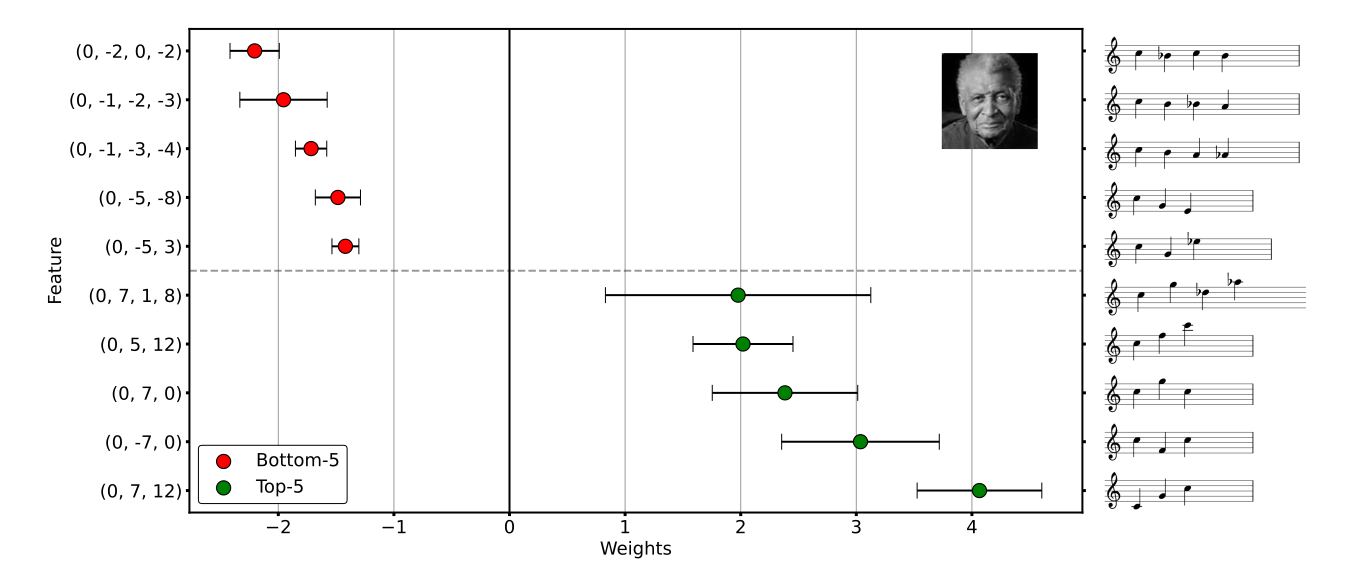
\includegraphics[width=1\textwidth]{figures/rsi_xai/figure_s4.pdf}
  \caption[Predictive melody features, Abdullah Ibrahim.]{Predictive melody features, Abdullah Ibrahim. This figure (and those following) shows standardised odds ratios obtained for every performer, following Figure \ref{fig:rsi_predictive_melody_features} in the full paper.}
\label{fig:rsi_sm_ibrahim_melody}
\end{figure}

\begin{figure}[!ht]
  \centering
  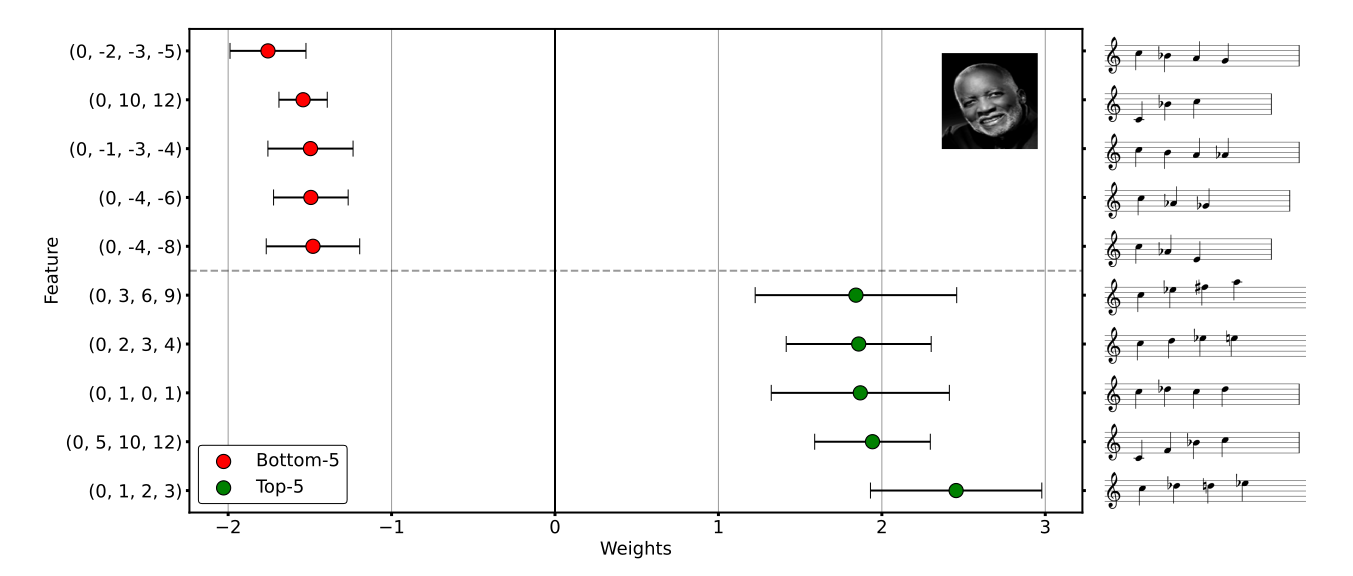
\includegraphics[width=1\textwidth]{figures/rsi_xai/figure_s5.pdf}
  \caption{Predictive melody features, Ahmad Jamal.}
\label{fig:rsi_sm_jamal_melody}
\end{figure}

\begin{figure}[!ht]
  \centering
  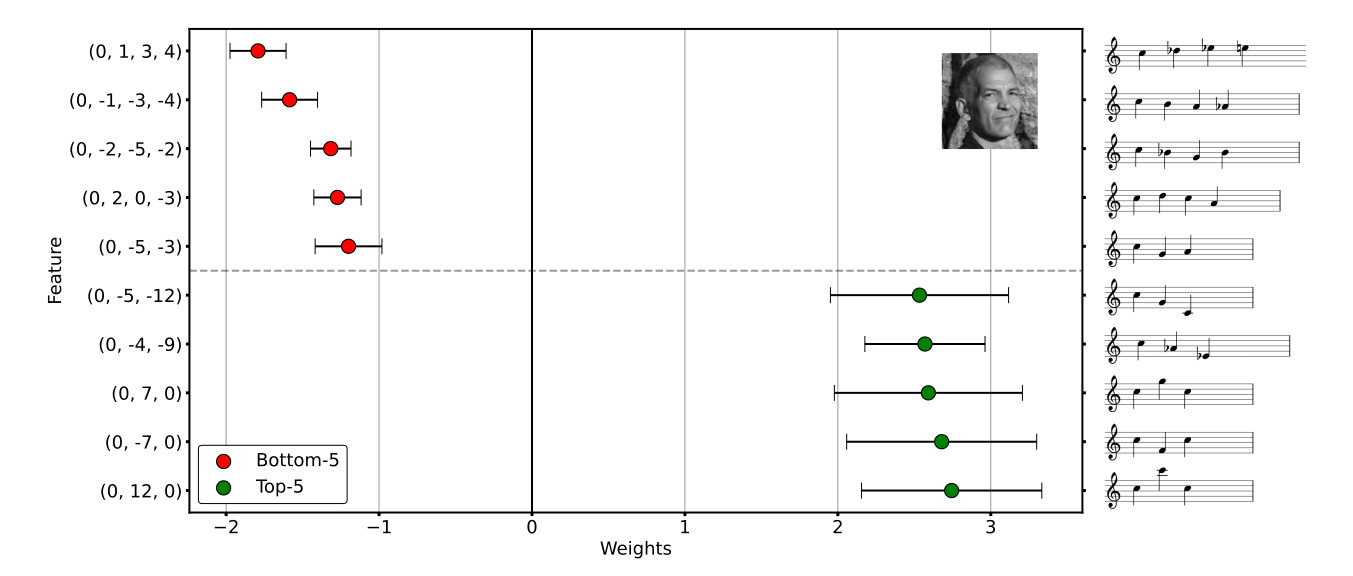
\includegraphics[width=1\textwidth]{figures/rsi_xai/figure_s6.pdf}
  \caption{Predictive melody features, Brad Mehldau.}
\label{fig:rsi_sm_mehldau_melody}
\end{figure}

\begin{figure}[!ht]
  \centering
  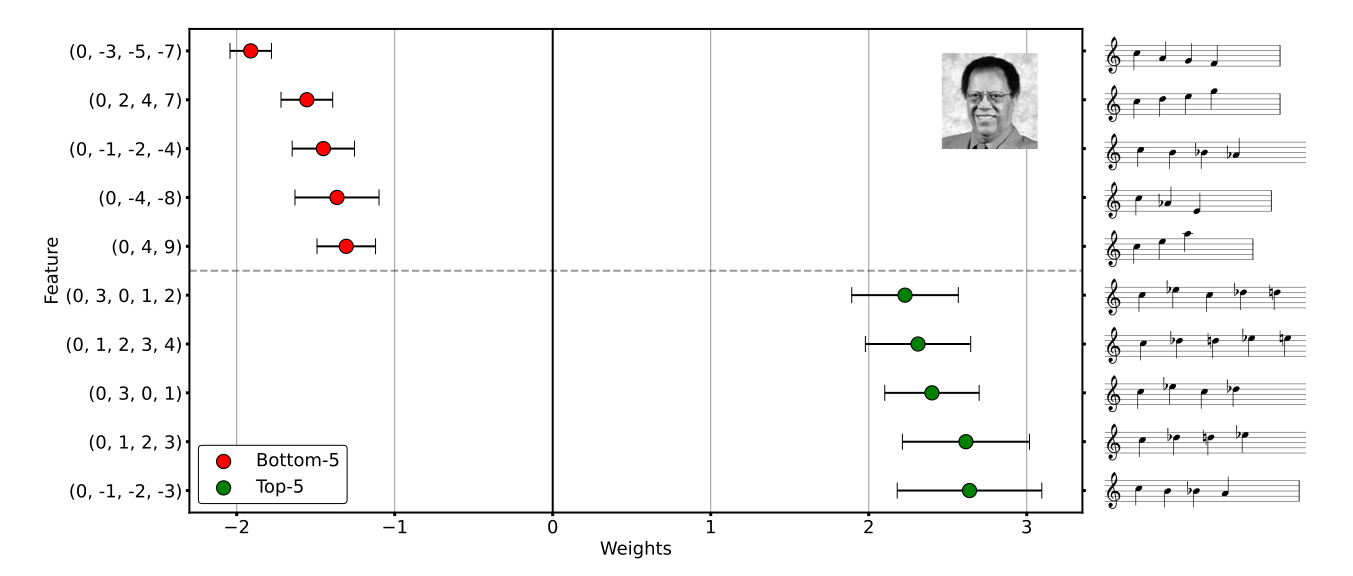
\includegraphics[width=1\textwidth]{figures/rsi_xai/figure_s7.pdf}
  \caption{Predictive melody features, Cedar Walton.}
\label{fig:rsi_sm_walton_melody}
\end{figure}

\begin{figure}[!ht]
  \centering
  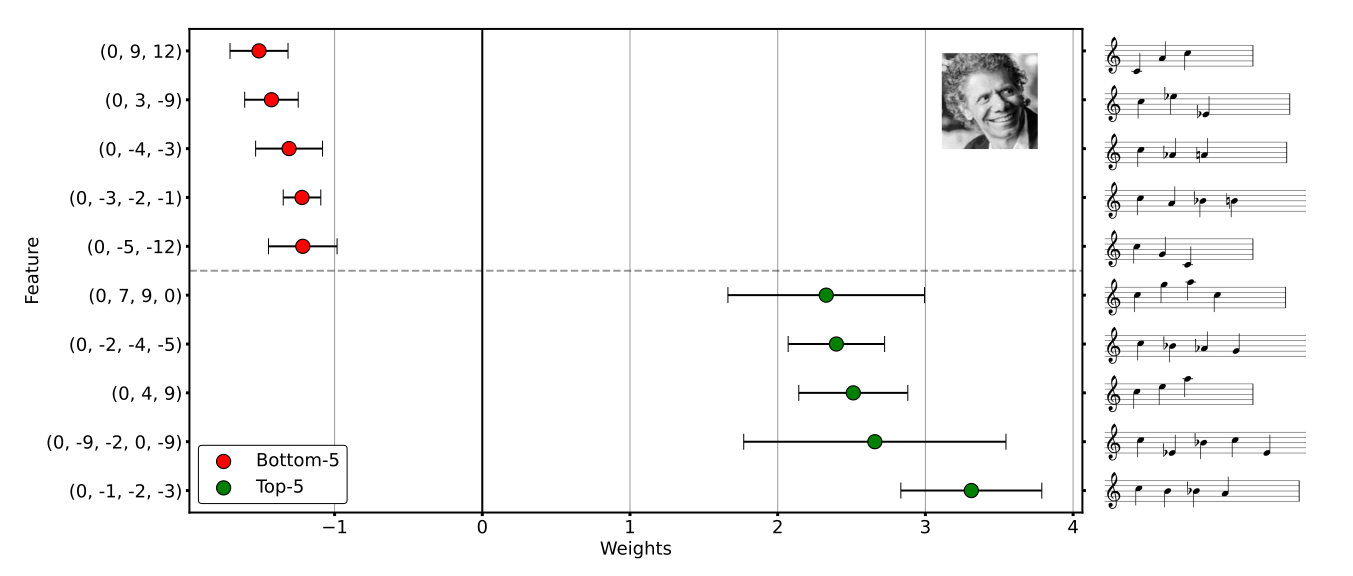
\includegraphics[width=1\textwidth]{figures/rsi_xai/figure_s8.pdf}
  \caption{Predictive melody features, Chick Corea.}
\label{fig:rsi_sm_corea_melody}
\end{figure}

\begin{figure}[!ht]
  \centering
  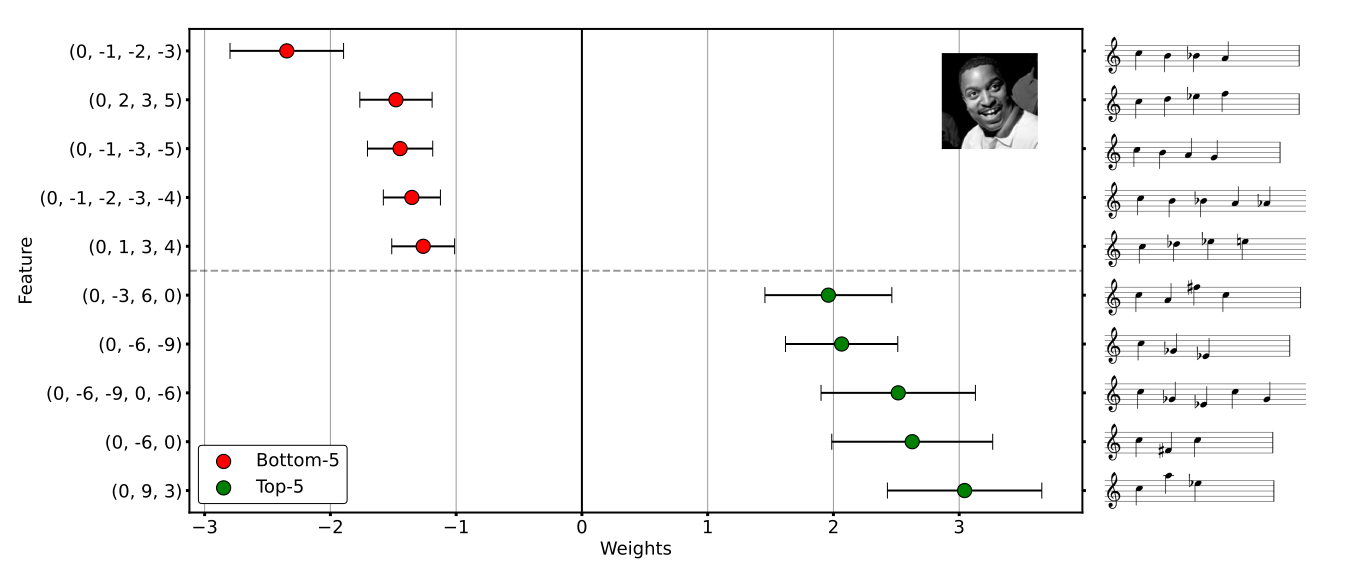
\includegraphics[width=1\textwidth]{figures/rsi_xai/figure_s9.pdf}
  \caption{Predictive melody features, Gene Harris.}
\label{fig:rsi_sm_harris_melody}
\end{figure}

\begin{figure}[!ht]
  \centering
  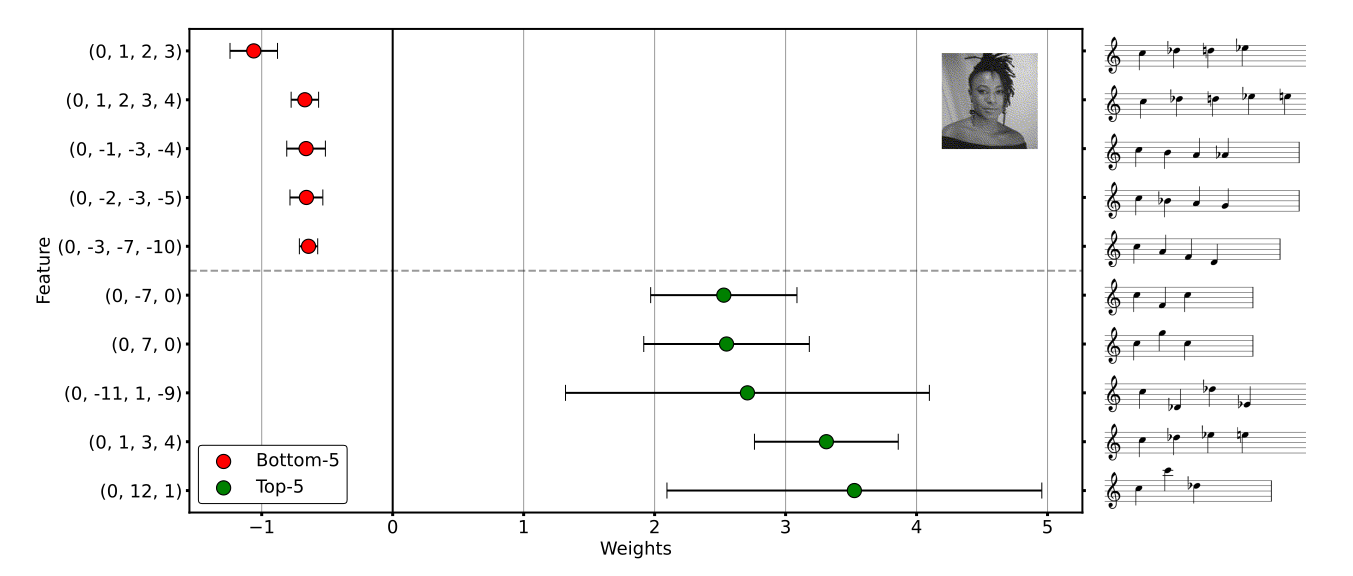
\includegraphics[width=1\textwidth]{figures/rsi_xai/figure_s10.pdf}
  \caption{Predictive melody features, Geri Allen.}
\label{fig:rsi_sm_allen_melody}
\end{figure}

\begin{figure}[!ht]
  \centering
  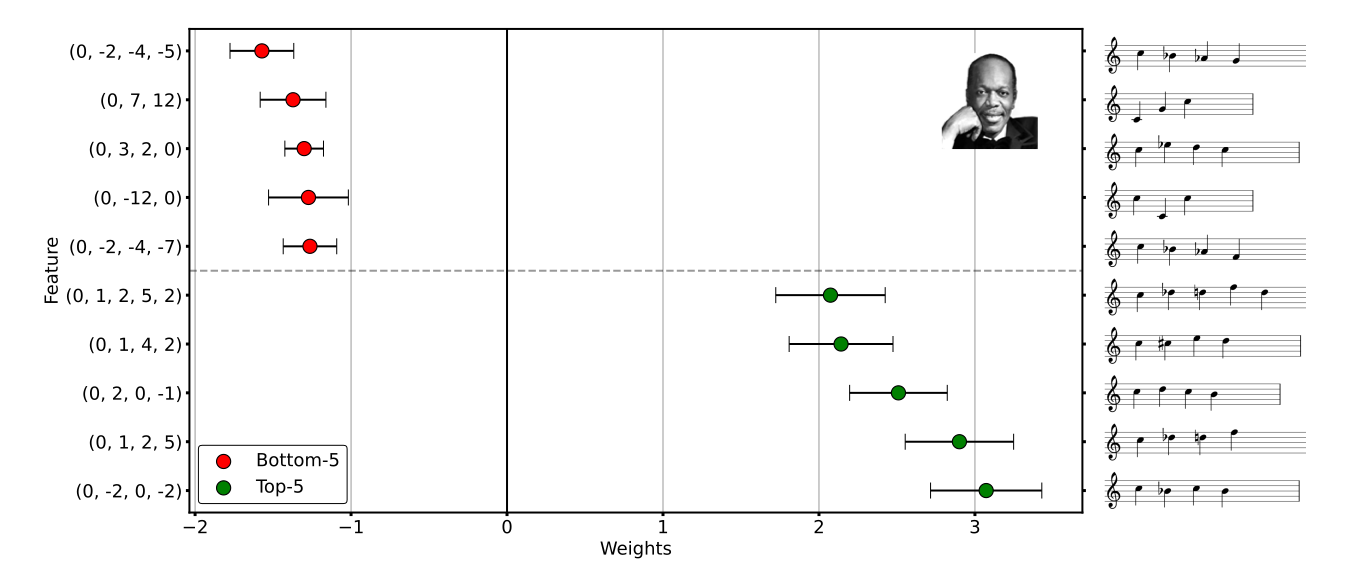
\includegraphics[width=1\textwidth]{figures/rsi_xai/figure_s11.pdf}
  \caption{Predictive melody features, Hank Jones.}
\label{fig:rsi_sm_jones_melody}
\end{figure}

\begin{figure}[!ht]
  \centering
  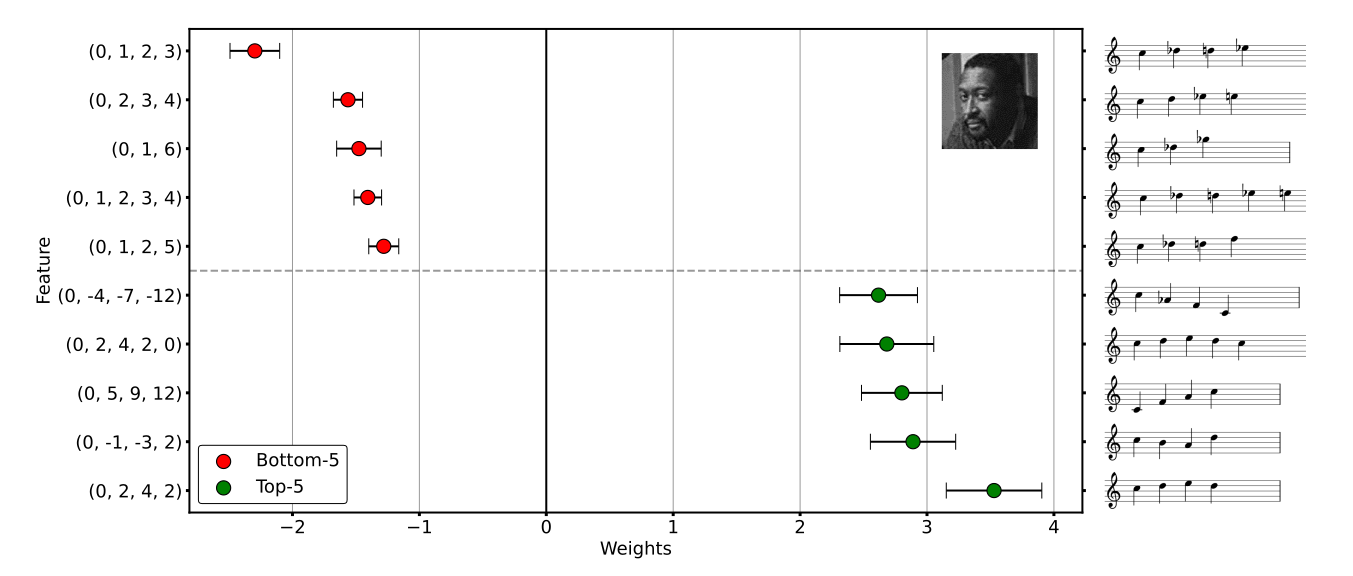
\includegraphics[width=1\textwidth]{figures/rsi_xai/figure_s12.pdf}
  \caption{Predictive melody features, John Hicks.}
\label{fig:rsi_sm_hicks_melody}
\end{figure}

\begin{figure}[!ht]
  \centering
  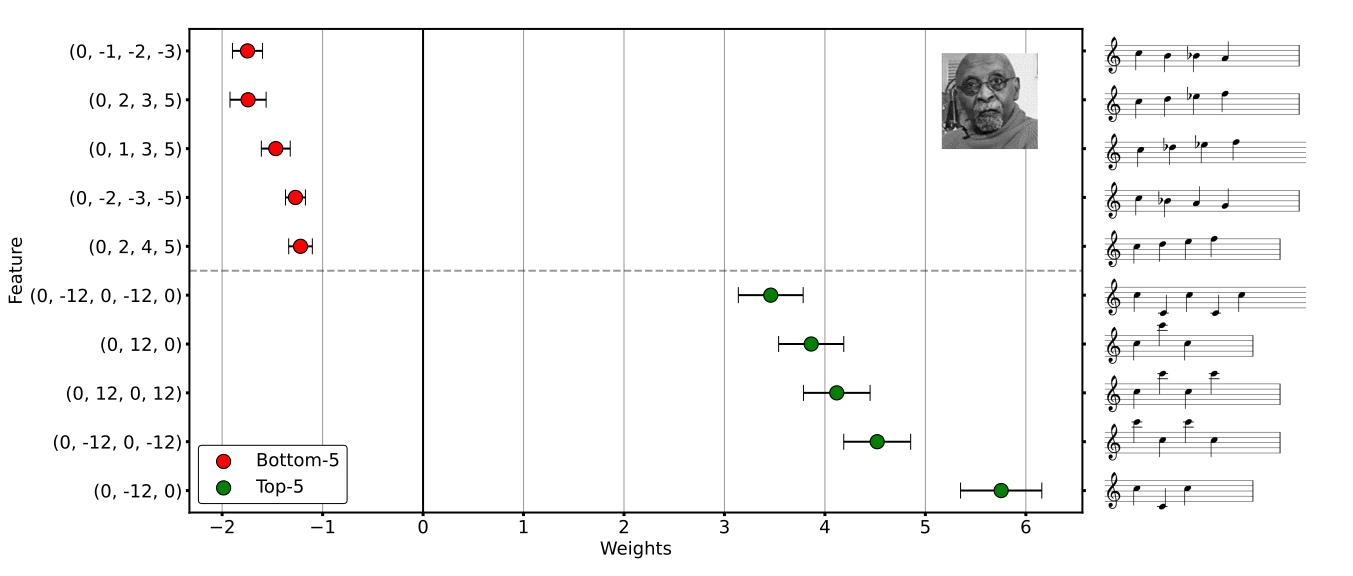
\includegraphics[width=1\textwidth]{figures/rsi_xai/figure_s13.pdf}
  \caption{Predictive melody features, Junior Mance.}
\label{fig:rsi_sm_mance_melody}
\end{figure}

\begin{figure}[!ht]
  \centering
  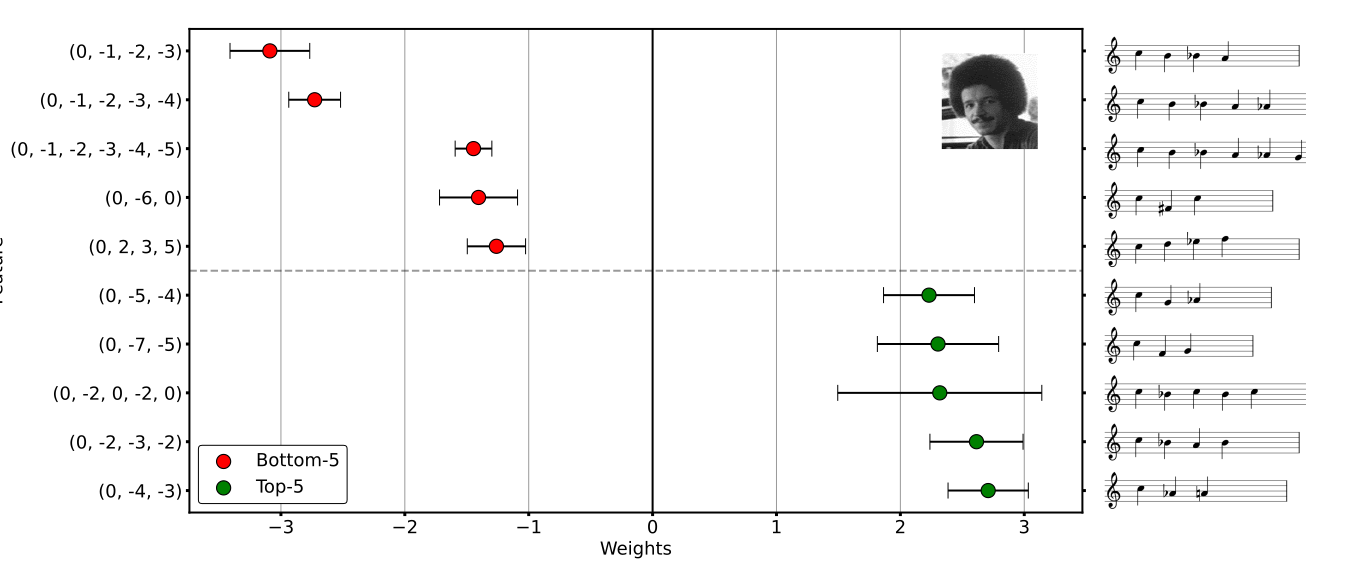
\includegraphics[width=1\textwidth]{figures/rsi_xai/figure_s14.pdf}
  \caption{Predictive melody features, Keith Jarrett.}
\label{fig:rsi_sm_jarrett_melody}
\end{figure}

\begin{figure}[!ht]
  \centering
  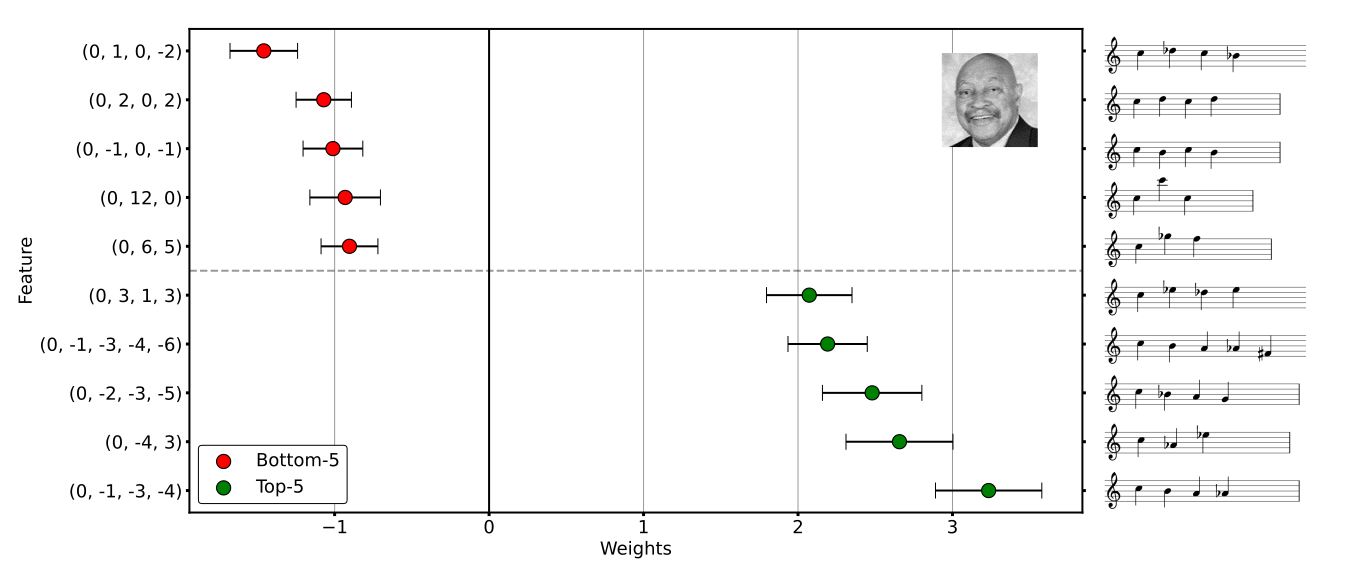
\includegraphics[width=1\textwidth]{figures/rsi_xai/figure_s15.pdf}
  \caption{Predictive melody features, Kenny Barron.}
\label{fig:rsi_sm_barron_melody}
\end{figure}

\begin{figure}[!ht]
  \centering
  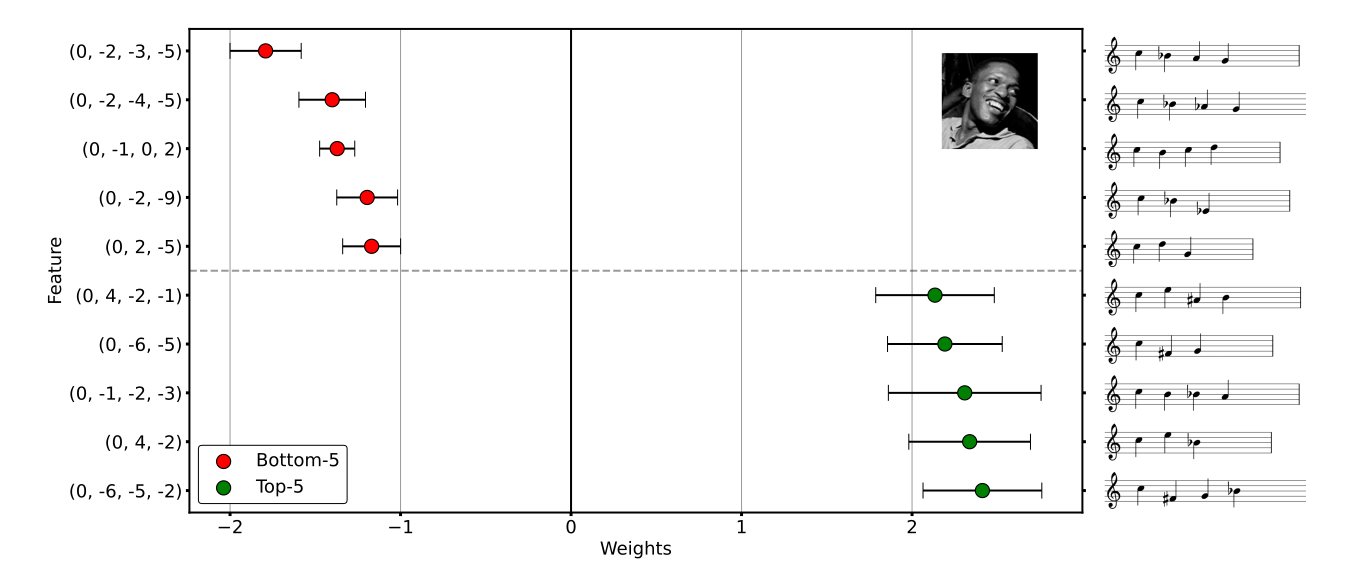
\includegraphics[width=1\textwidth]{figures/rsi_xai/figure_s16.pdf}
  \caption{Predictive melody features, Kenny Drew.}
\label{fig:rsi_sm_drew_melody}
\end{figure}

\begin{figure}[!ht]
  \centering
  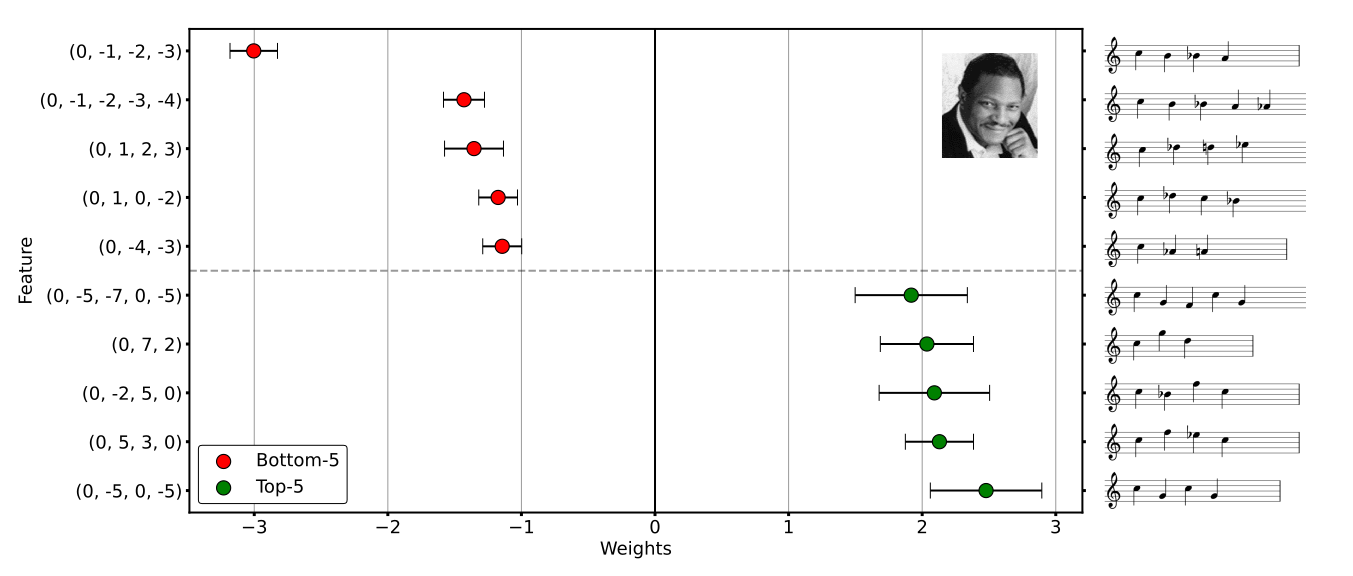
\includegraphics[width=1\textwidth]{figures/rsi_xai/figure_s17.pdf}
  \caption{Predictive melody features, McCoy Tyner.}
\label{fig:rsi_sm_tyner_melody}
\end{figure}

\begin{figure}[!ht]
  \centering
  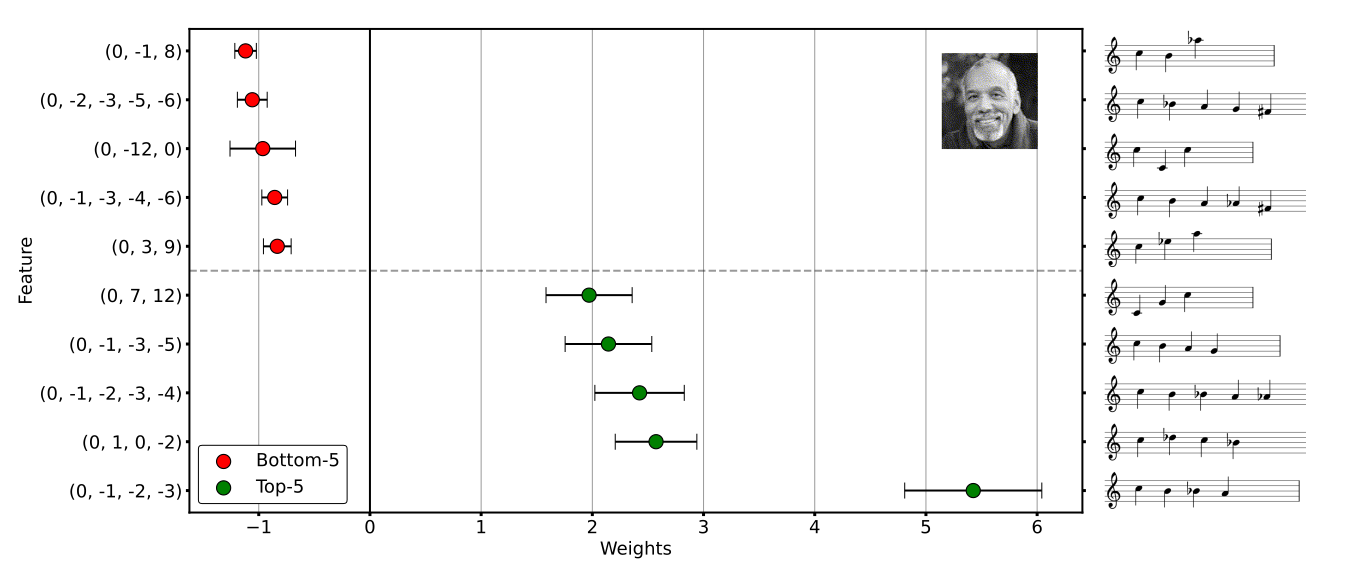
\includegraphics[width=1\textwidth]{figures/rsi_xai/figure_s18.pdf}
  \caption{Predictive melody features, Stanley Cowell.}
\label{fig:rsi_sm_cowell_melody}
\end{figure}

\begin{figure}[!ht]
  \centering
  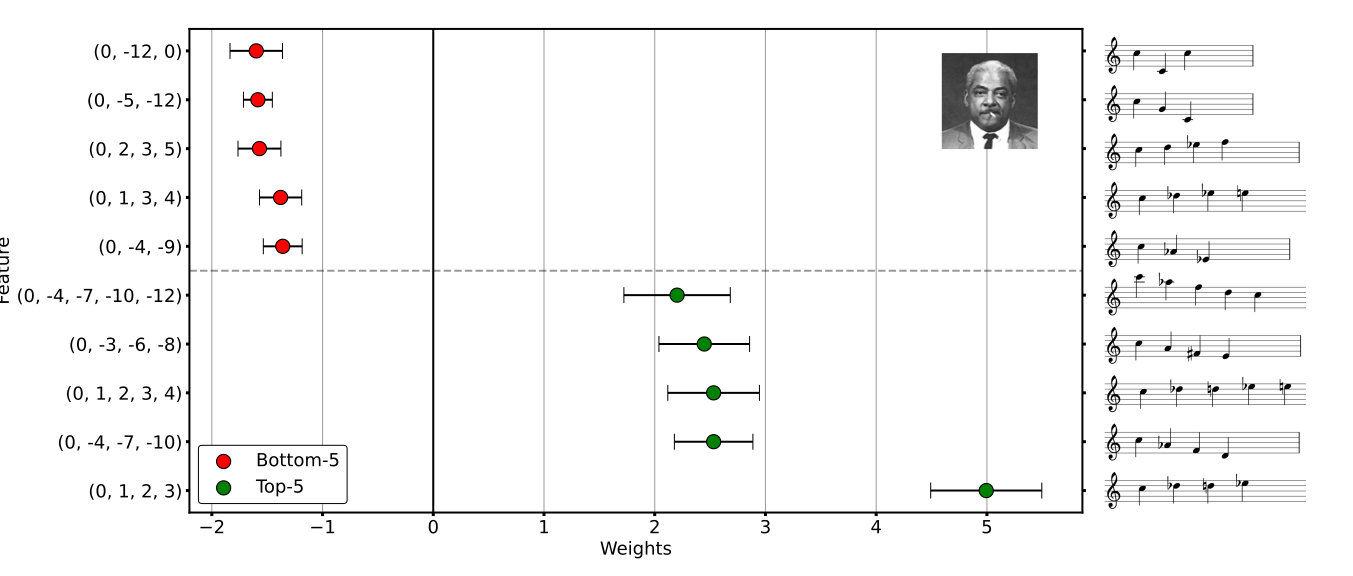
\includegraphics[width=1\textwidth]{figures/rsi_xai/figure_s19.pdf}
  \caption{Predictive melody features, Teddy Wilson.}
\label{fig:rsi_sm_wilson_melody}
\end{figure}

\begin{figure}[!ht]
  \centering
  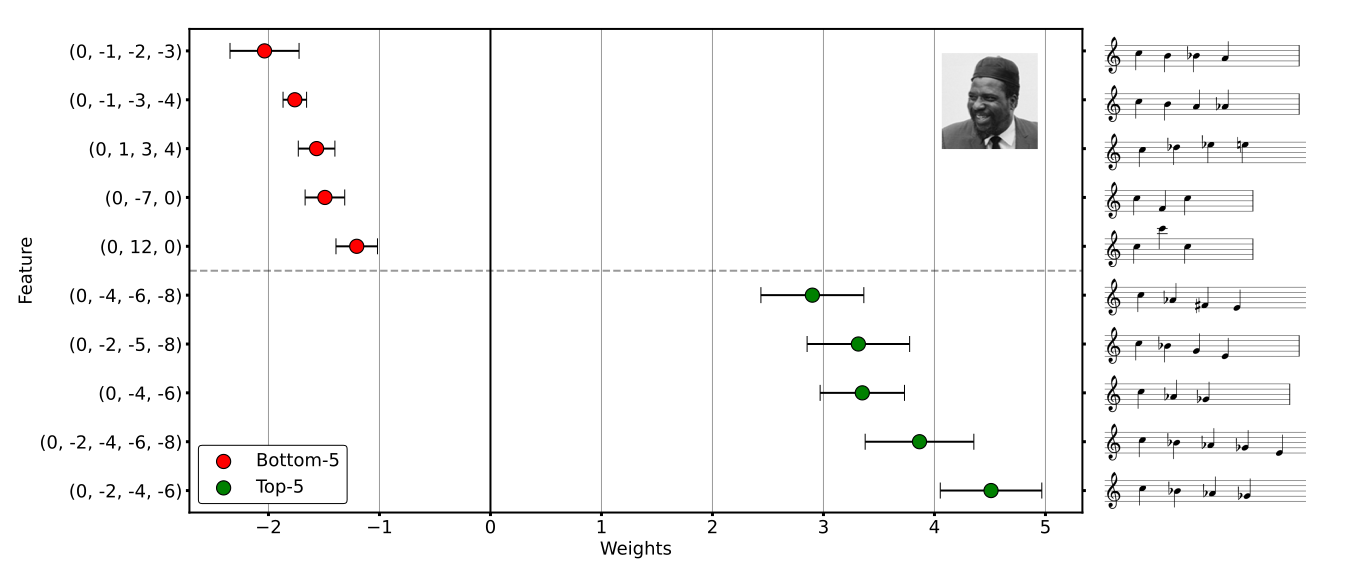
\includegraphics[width=1\textwidth]{figures/rsi_xai/figure_s20.pdf}
  \caption{Predictive melody features, Thelonious Monk.}
\label{fig:rsi_sm_monk_melody}
\end{figure}

\begin{figure}[!ht]
  \centering
  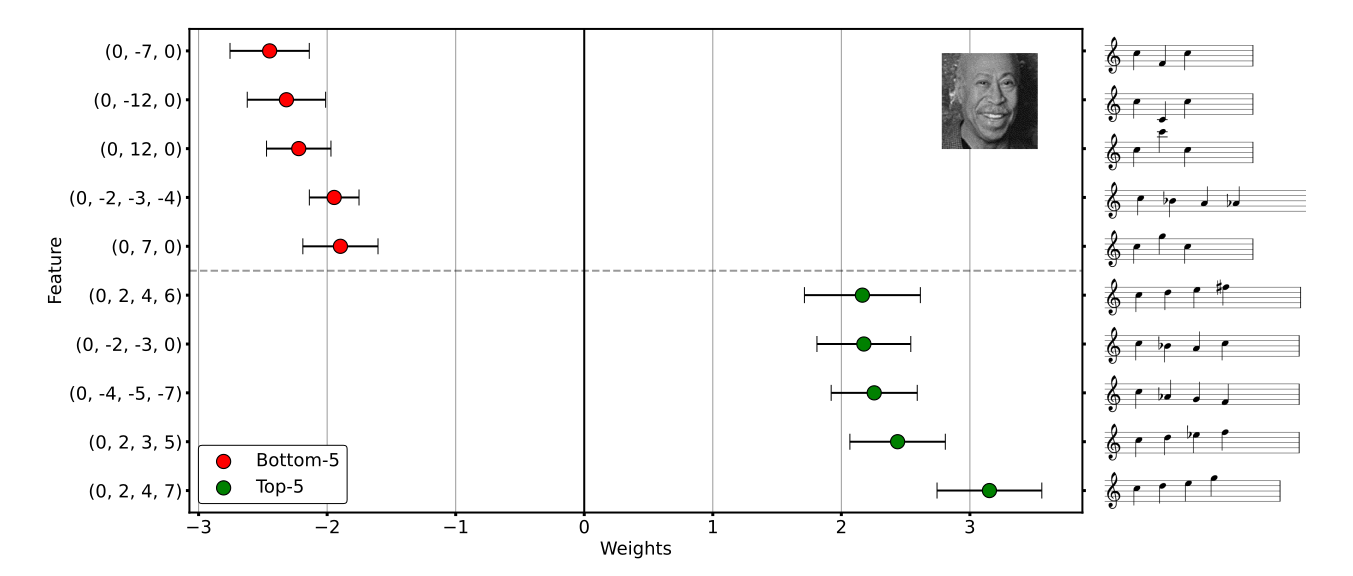
\includegraphics[width=1\textwidth]{figures/rsi_xai/figure_s21.pdf}
  \caption{Predictive melody features, Tommy Flanagan.}
\label{fig:rsi_sm_flanagan_melody}
\end{figure}

\begin{figure}[!ht]
  \centering
  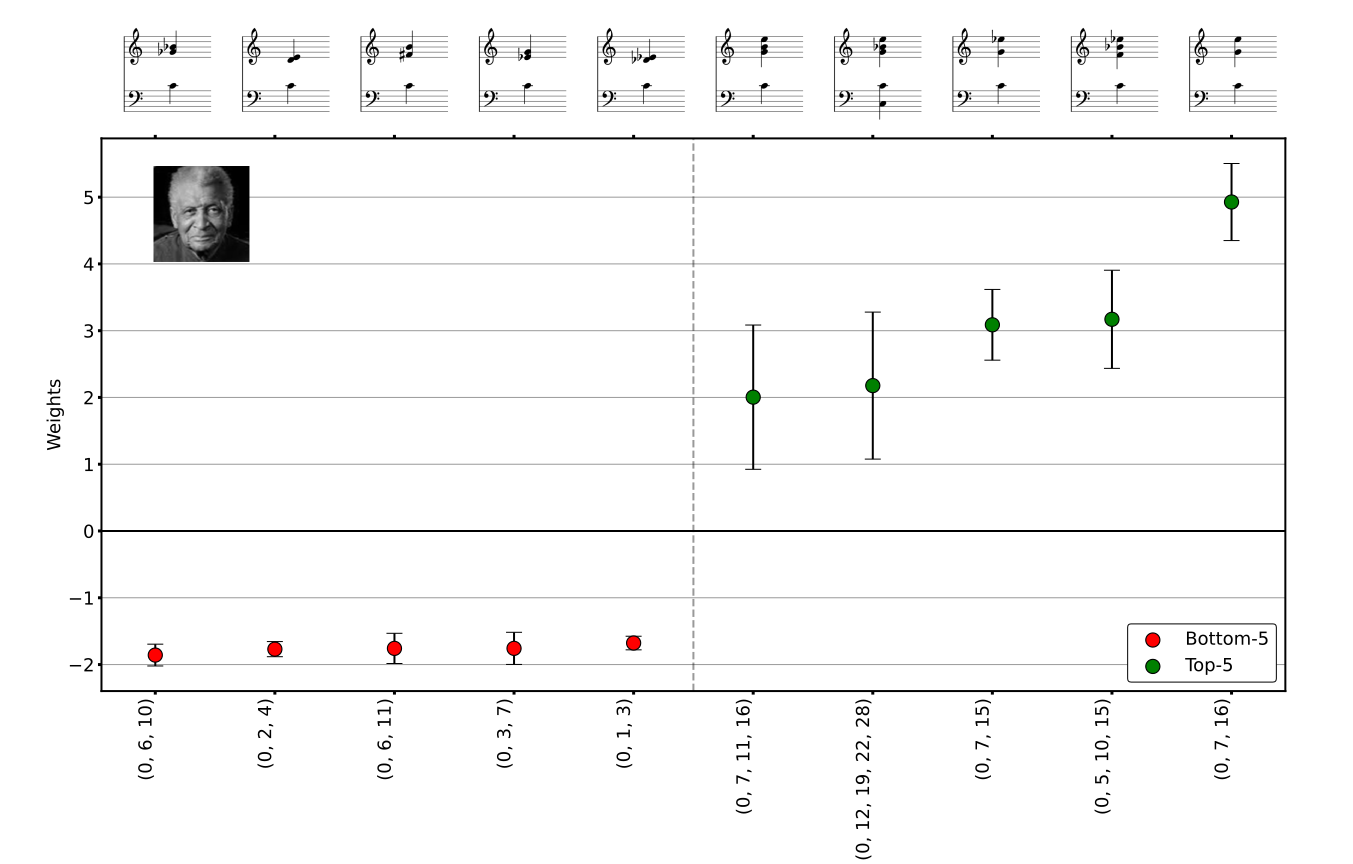
\includegraphics[width=1\textwidth]{figures/rsi_xai/figure_s22.pdf}
  \caption[Predictive harmony features, Abdullah Ibrahim.]{Predictive harmony features, Abdullah Ibrahim. Note that the direction of the axis in these figures is reversed compared to the previous figures, in order to accommodate the ``grand staff'' notation.}
\label{fig:rsi_sm_ibrahim_harmony}
\end{figure}

\begin{figure}[!ht]
  \centering
  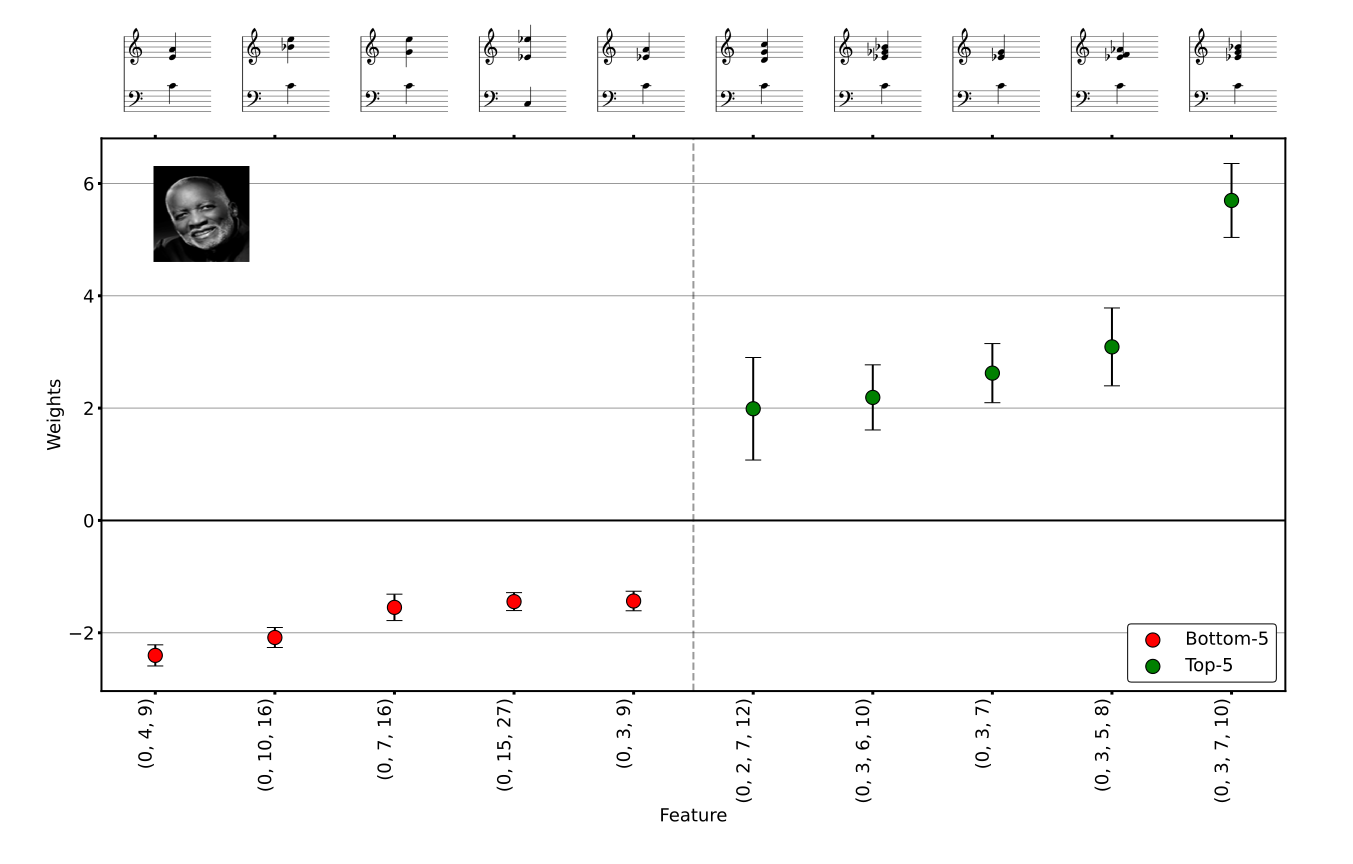
\includegraphics[width=1\textwidth]{figures/rsi_xai/figure_s23.pdf}
  \caption{Predictive harmony features, Ahmad Jamal.}
\label{fig:rsi_sm_jamal_harmony}
\end{figure}

\begin{figure}[!ht]
  \centering
  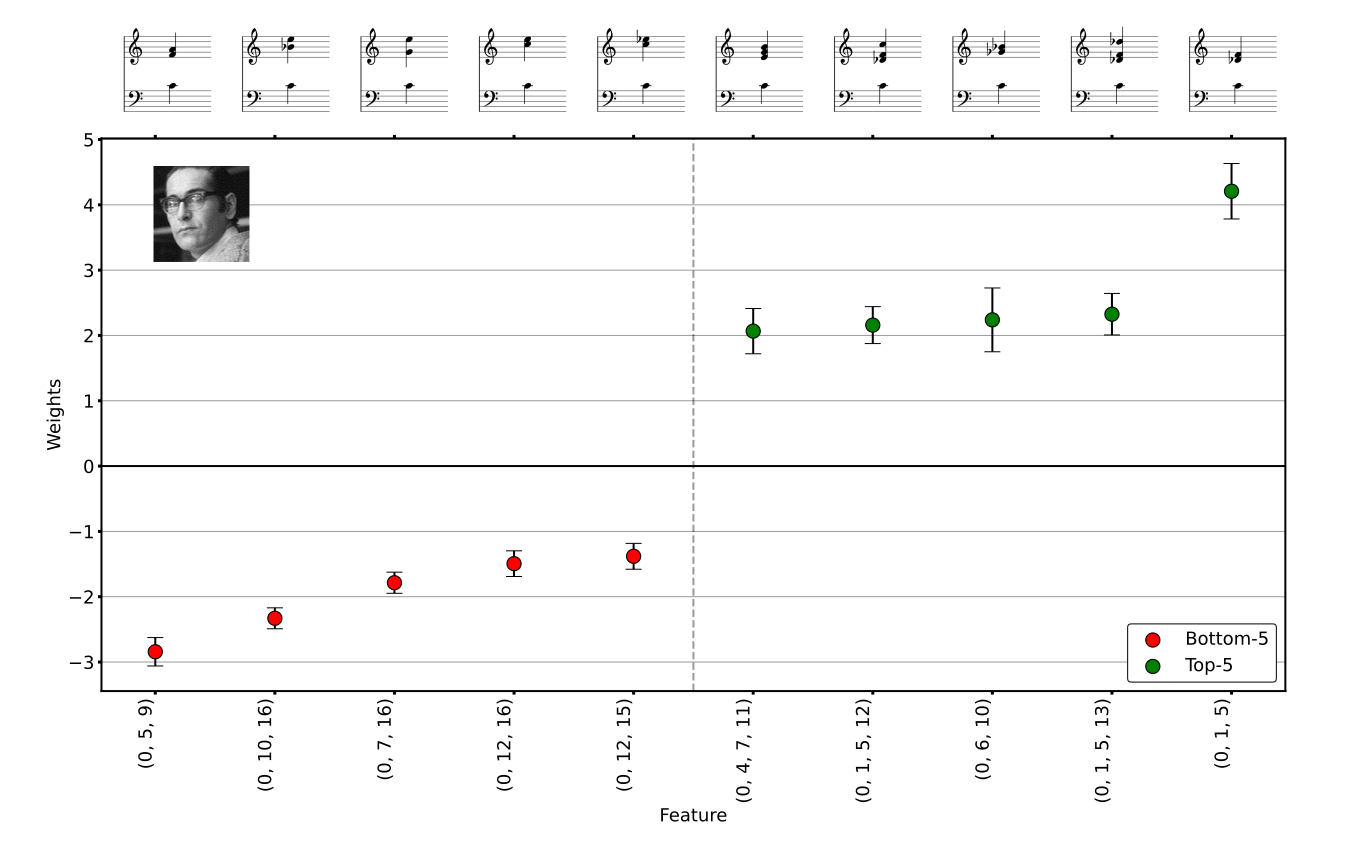
\includegraphics[width=1\textwidth]{figures/rsi_xai/figure_s24.pdf}
  \caption{Predictive harmony features, Bill Evans.}
\label{fig:rsi_sm_evans_harmony}
\end{figure}

\begin{figure}[!ht]
  \centering
  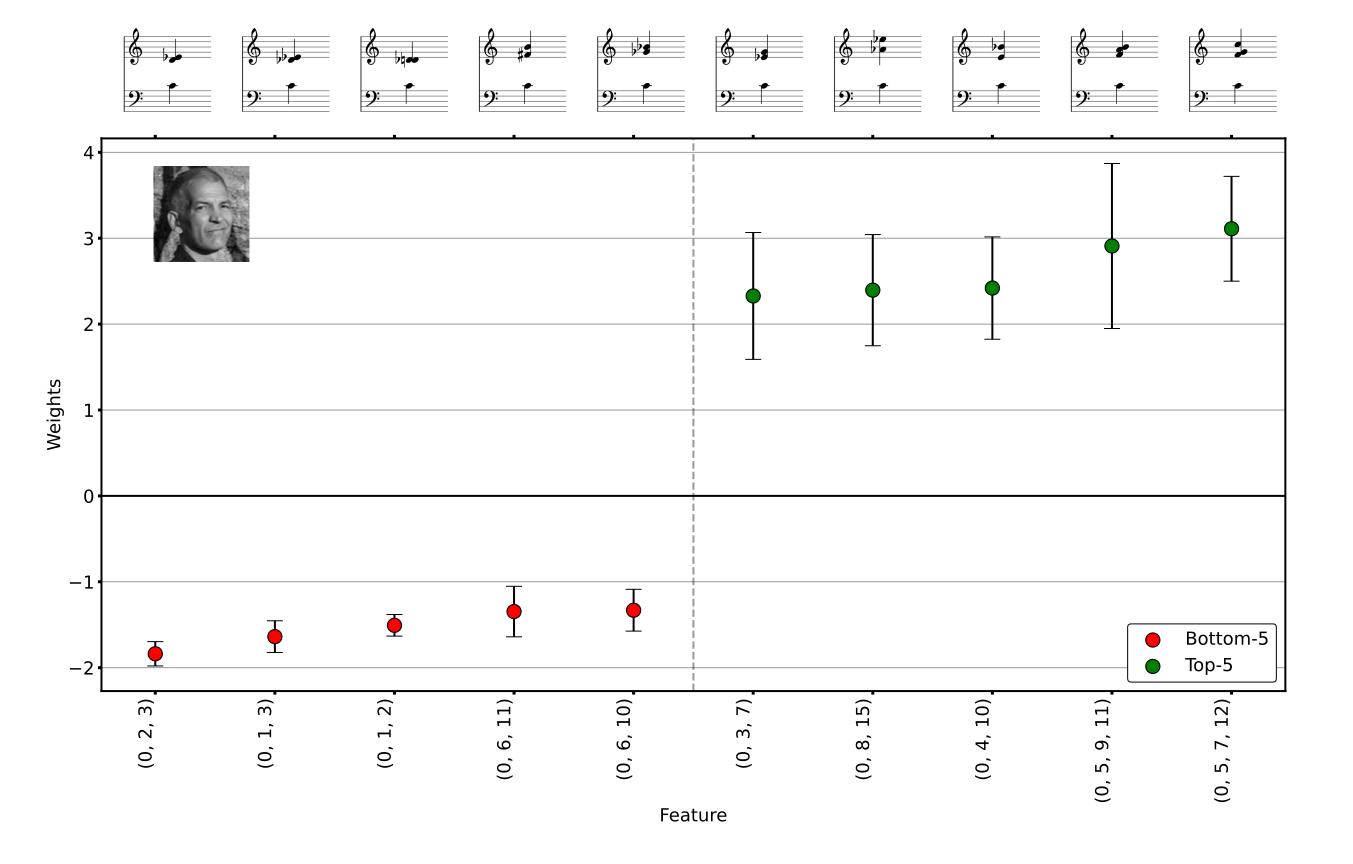
\includegraphics[width=1\textwidth]{figures/rsi_xai/figure_s25.pdf}
  \caption{Predictive harmony features, Brad Mehldau.}
\label{fig:rsi_sm_mehldau_harmony}
\end{figure}

\begin{figure}[!ht]
  \centering
  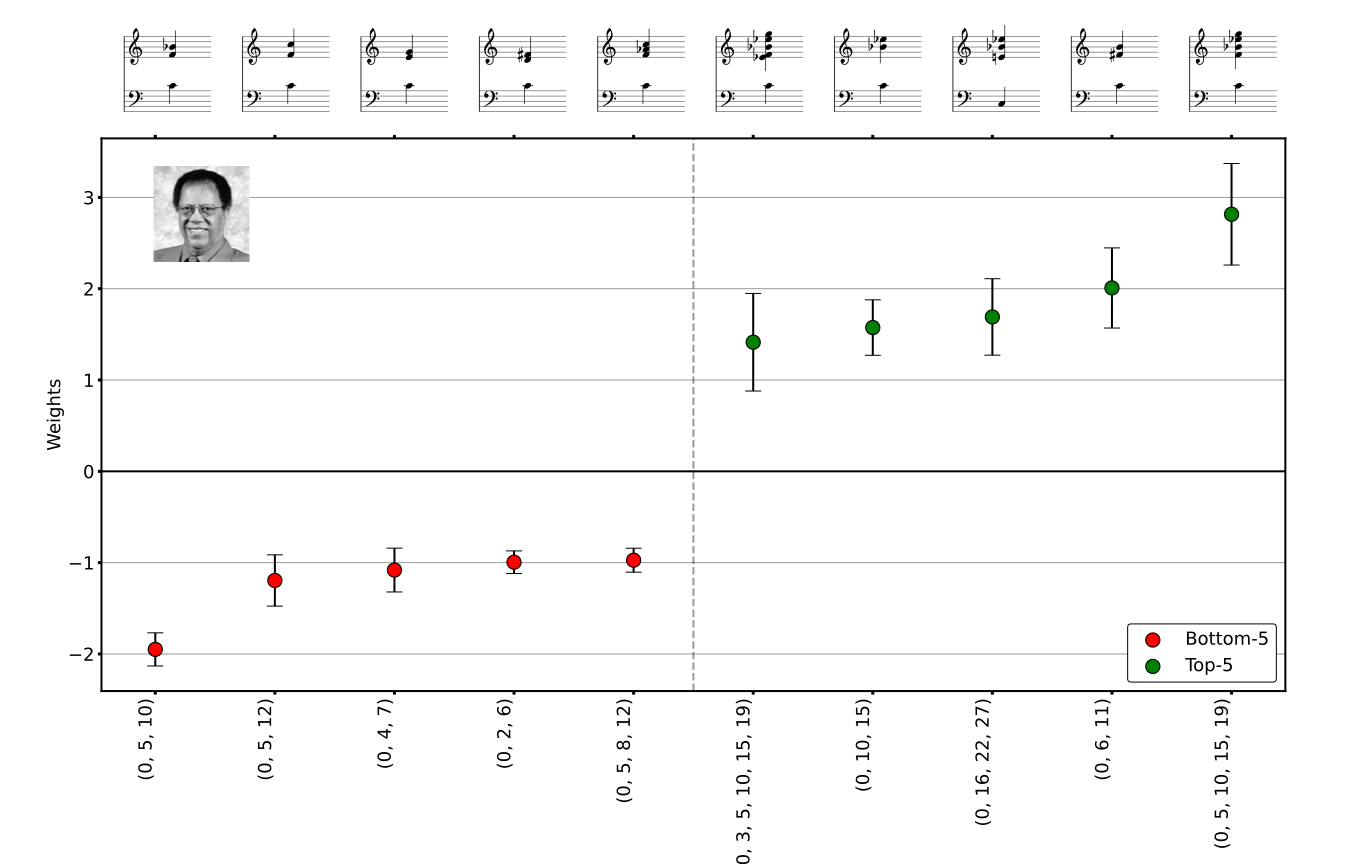
\includegraphics[width=1\textwidth]{figures/rsi_xai/figure_s26.pdf}
  \caption{Predictive harmony features, Cedar Walton.}
\label{fig:rsi_sm_walton_harmony}
\end{figure}

\begin{figure}[!ht]
  \centering
  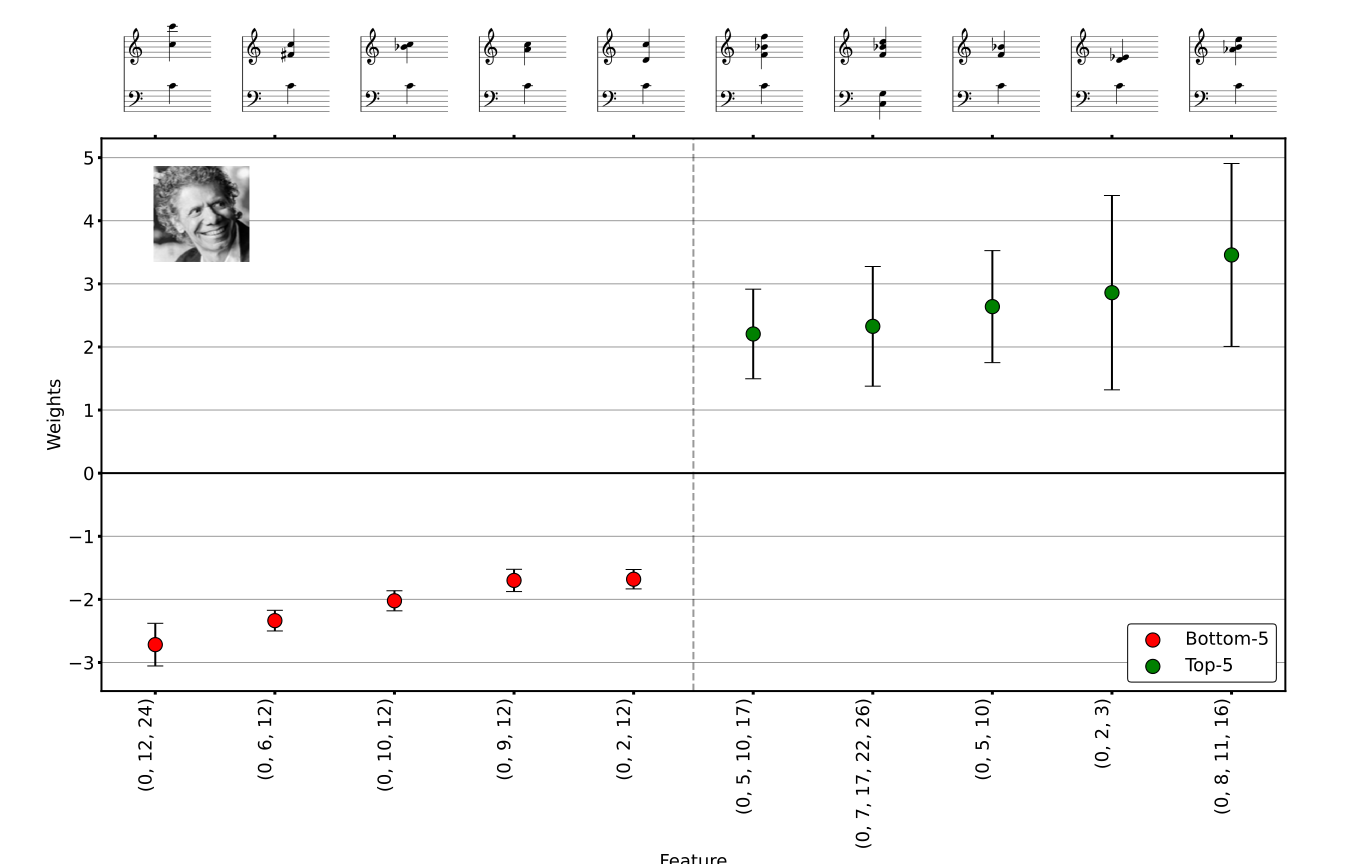
\includegraphics[width=1\textwidth]{figures/rsi_xai/figure_s27.pdf}
  \caption{Predictive harmony features, Chick Corea.}
\label{fig:rsi_sm_corea_harmony}
\end{figure}

\begin{figure}[!ht]
  \centering
  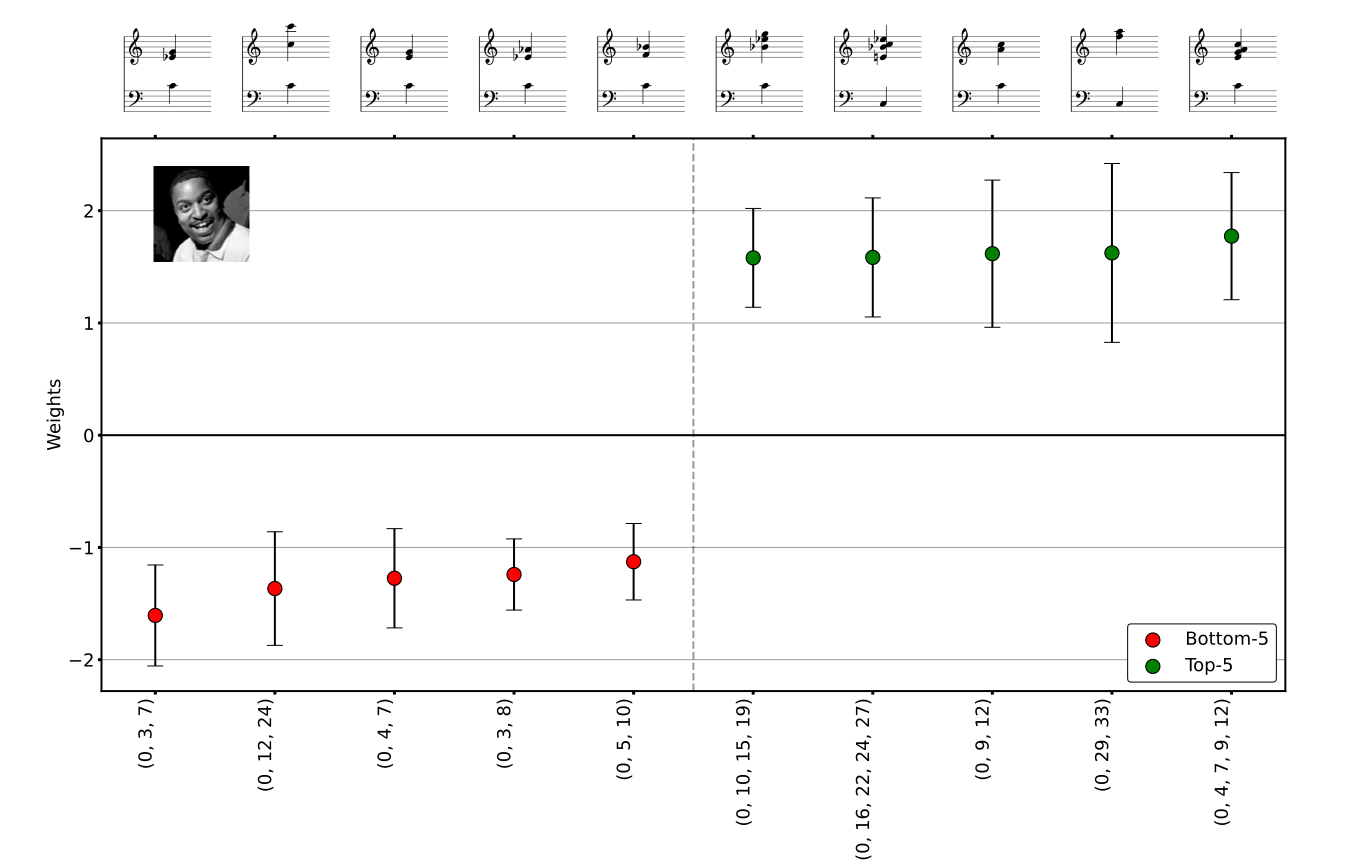
\includegraphics[width=1\textwidth]{figures/rsi_xai/figure_s28.pdf}
  \caption{Predictive harmony features, Gene Harris.}
\label{fig:rsi_sm_harris_harmony}
\end{figure}

\begin{figure}[!ht]
  \centering
  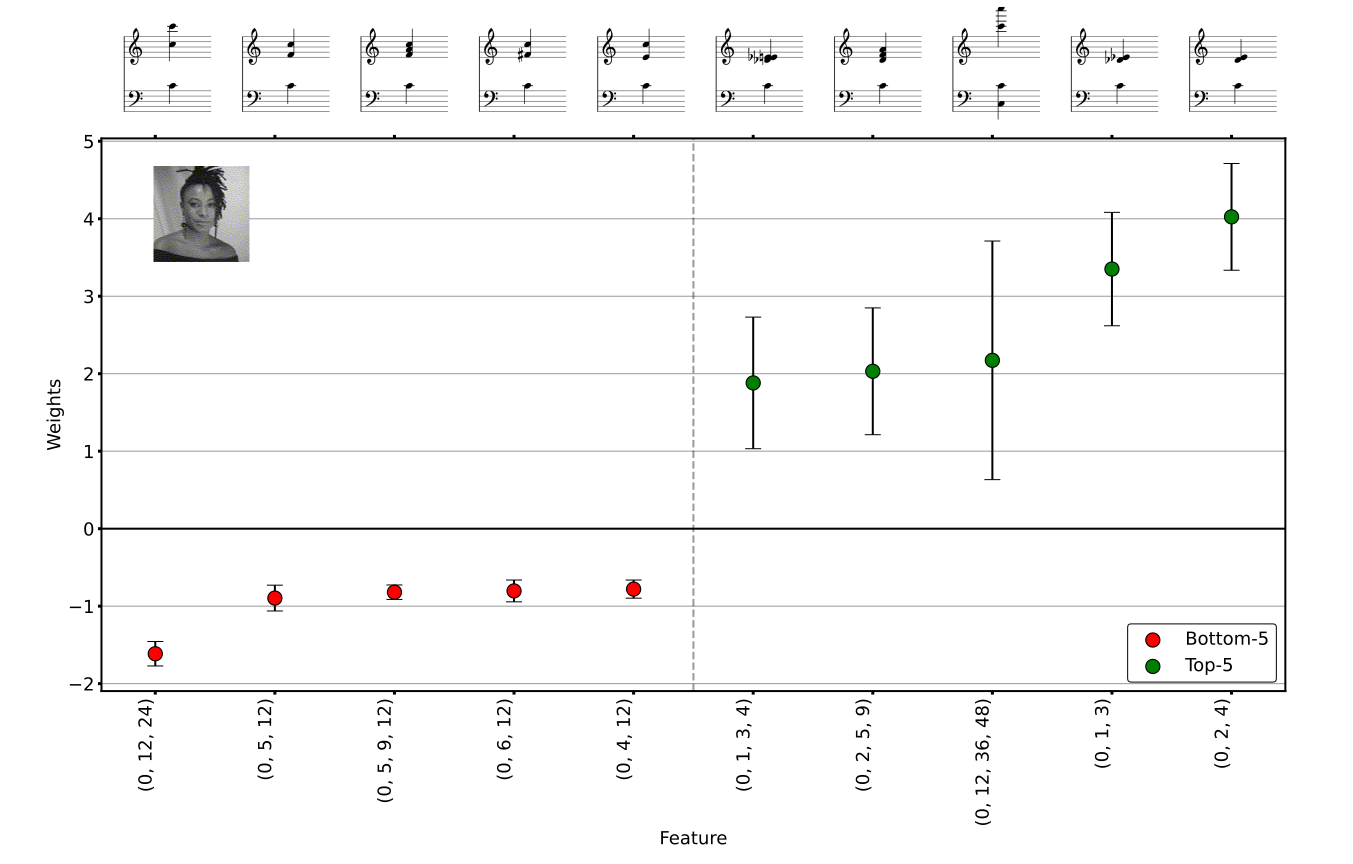
\includegraphics[width=1\textwidth]{figures/rsi_xai/figure_s29.pdf}
  \caption{Predictive harmony features, Geri Allen.}
\label{fig:rsi_sm_allen_harmony}
\end{figure}

\begin{figure}[!ht]
  \centering
  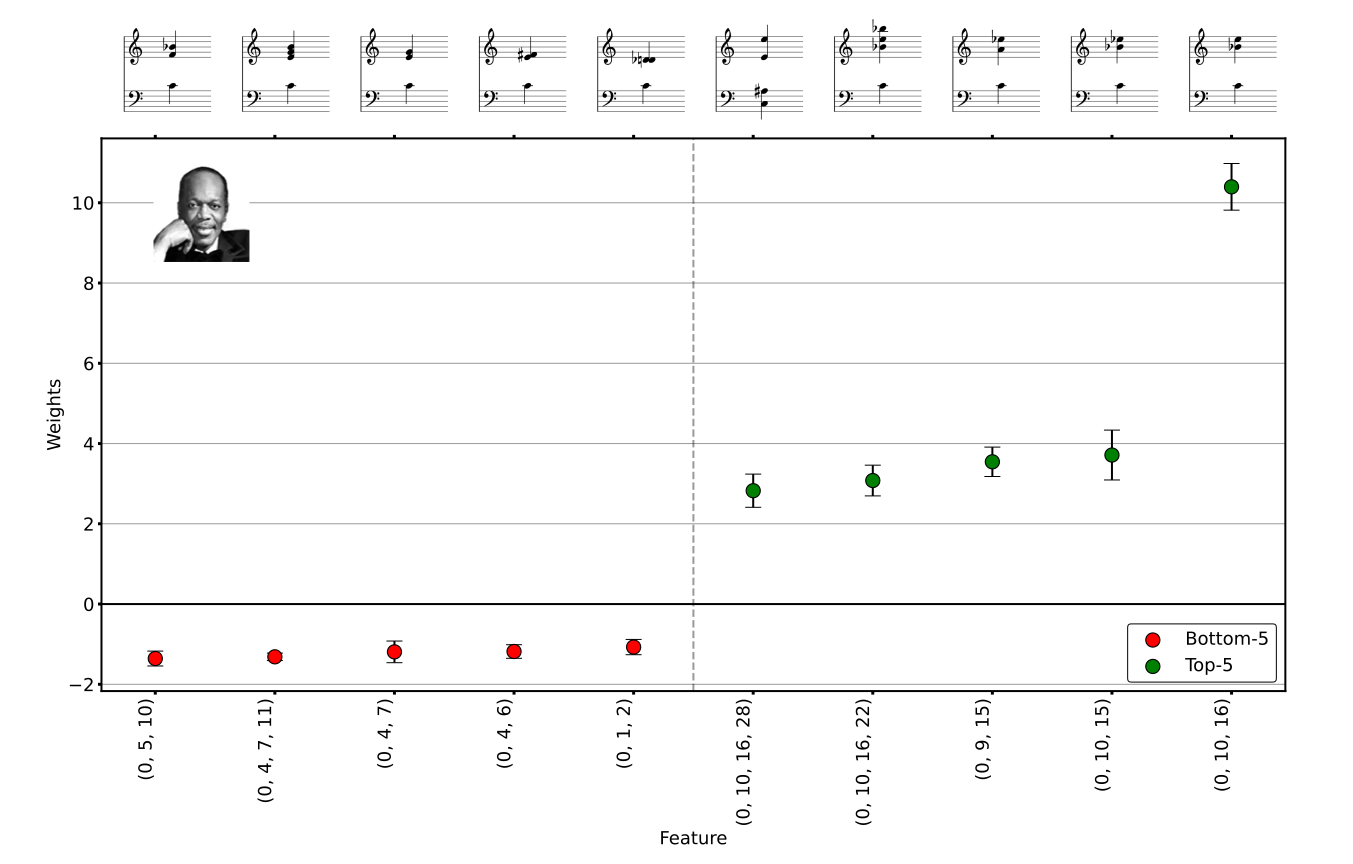
\includegraphics[width=1\textwidth]{figures/rsi_xai/figure_s30.pdf}
  \caption{Predictive harmony features, Hank Jones.}
\label{fig:rsi_sm_jones_harmony}
\end{figure}

\begin{figure}[!ht]
  \centering
  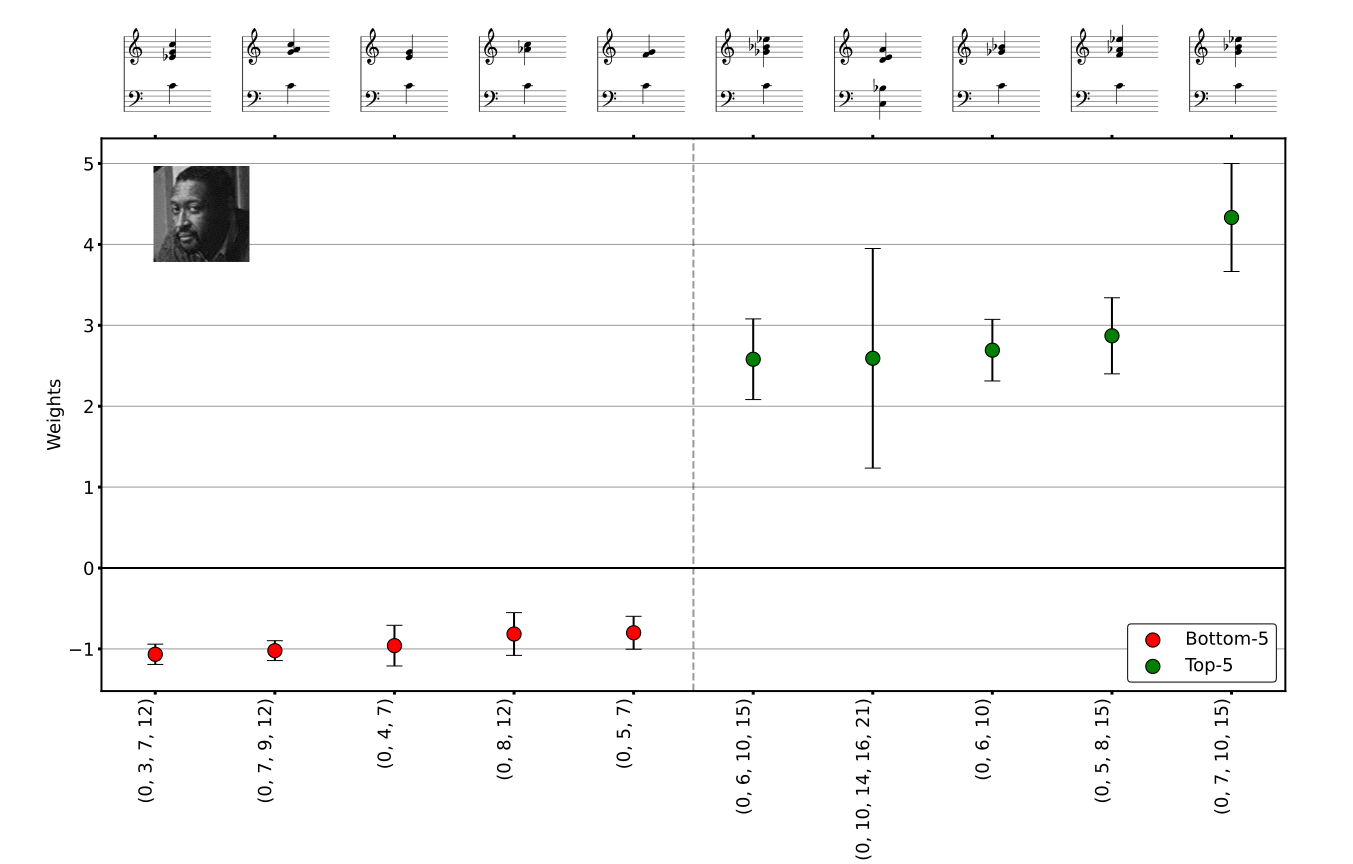
\includegraphics[width=1\textwidth]{figures/rsi_xai/figure_s31.pdf}
  \caption{Predictive harmony features, John Hicks.}
\label{fig:rsi_sm_hicks_harmony}
\end{figure}

\begin{figure}[!ht]
  \centering
  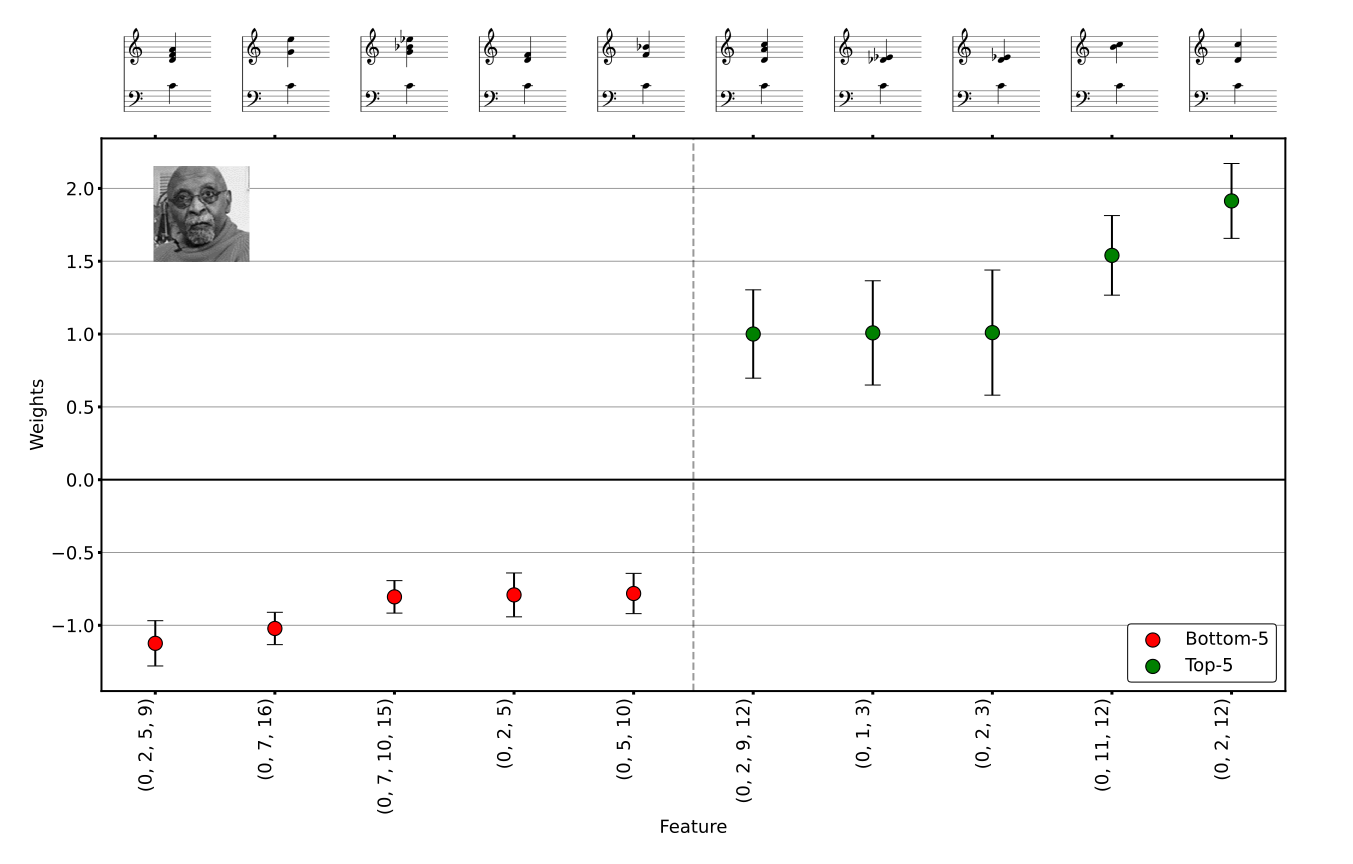
\includegraphics[width=1\textwidth]{figures/rsi_xai/figure_s32.pdf}
  \caption{Predictive harmony features, Junior Mance.}
\label{fig:rsi_sm_mance_harmony}
\end{figure}

\begin{figure}[!ht]
  \centering
  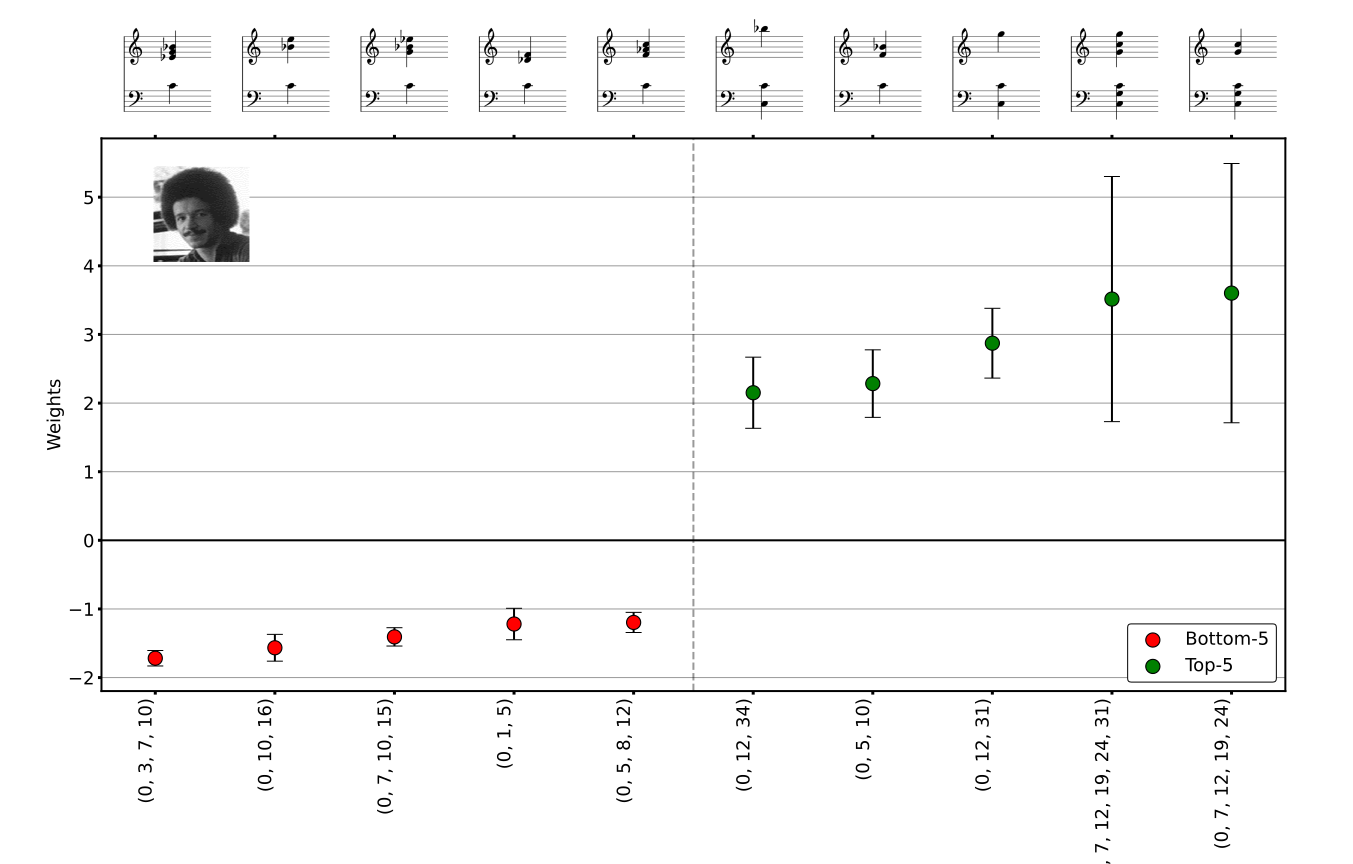
\includegraphics[width=1\textwidth]{figures/rsi_xai/figure_s33.pdf}
  \caption{Predictive harmony features, Keith Jarrett.}
\label{fig:rsi_sm_jarrett_harmony}
\end{figure}

\begin{figure}[!ht]
  \centering
  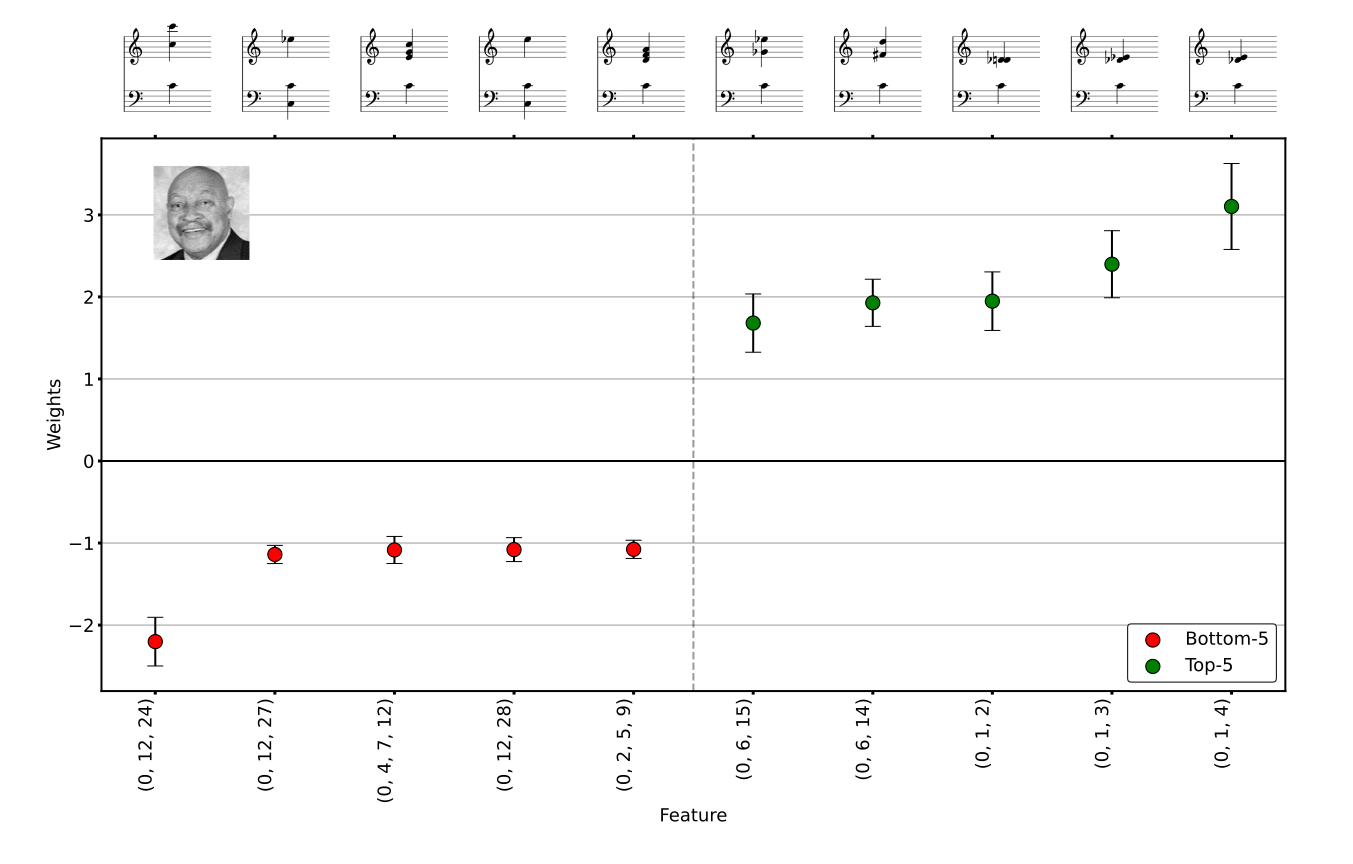
\includegraphics[width=1\textwidth]{figures/rsi_xai/figure_s34.pdf}
  \caption{Predictive harmony features, Kenny Barron.}
\label{fig:rsi_sm_barron_harmony}
\end{figure}

\begin{figure}[!ht]
  \centering
  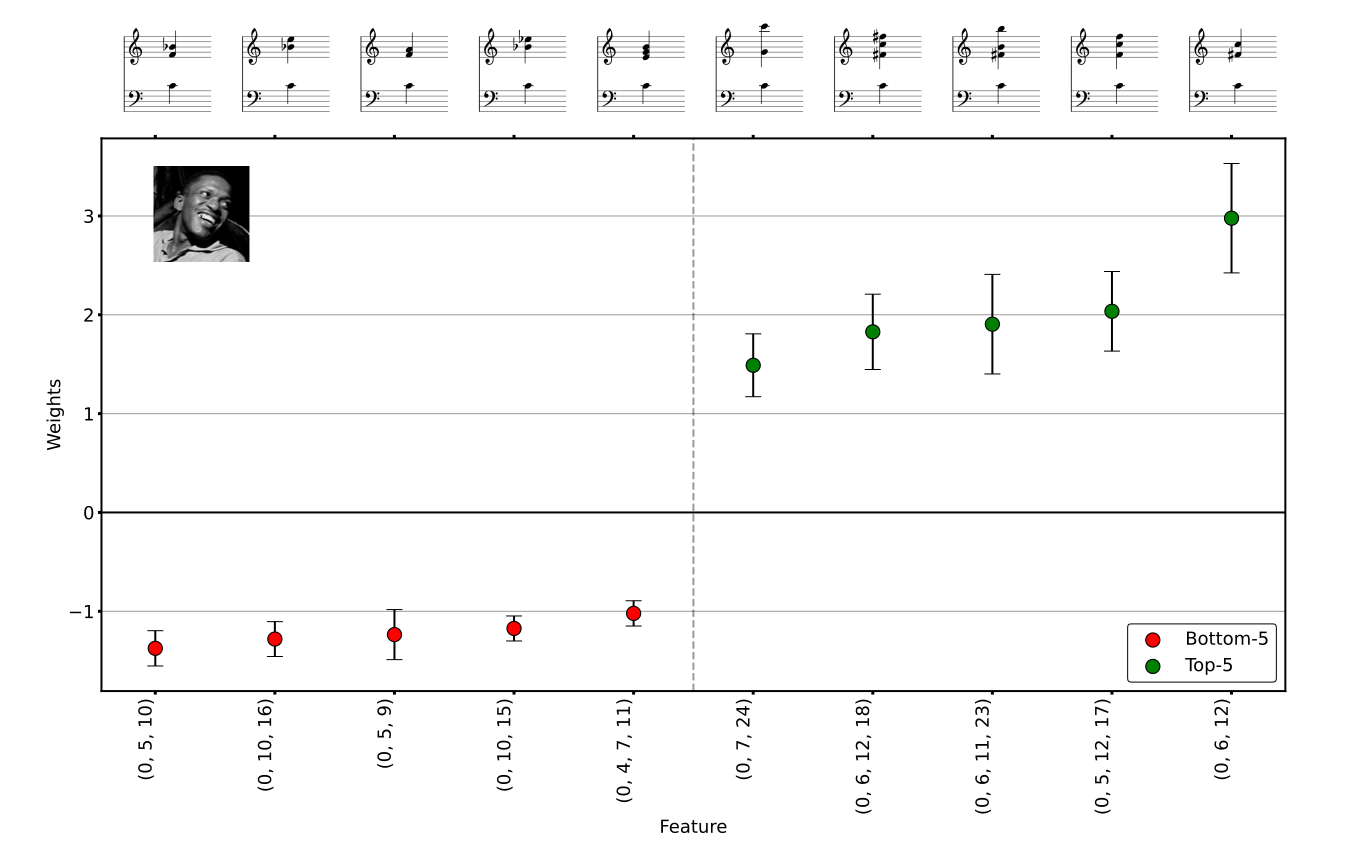
\includegraphics[width=1\textwidth]{figures/rsi_xai/figure_s35.pdf}
  \caption{Predictive harmony features, Kenny Drew.}
\label{fig:rsi_sm_drew_harmony}
\end{figure}

\begin{figure}[!ht]
  \centering
  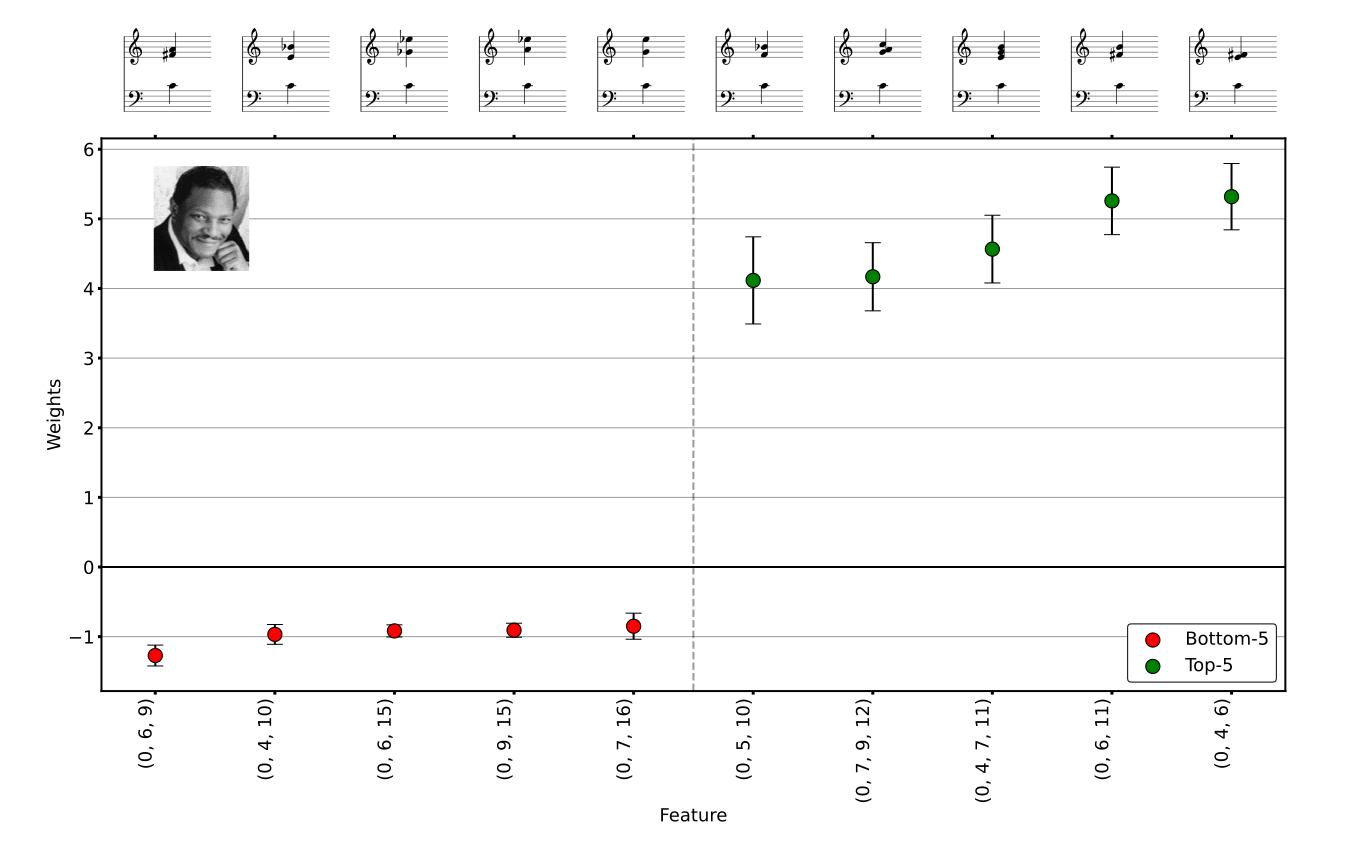
\includegraphics[width=1\textwidth]{figures/rsi_xai/figure_s36.pdf}
  \caption{Predictive harmony features, McCoy Tyner.}
\label{fig:rsi_sm_tyner_harmony}
\end{figure}

\begin{figure}[!ht]
  \centering
  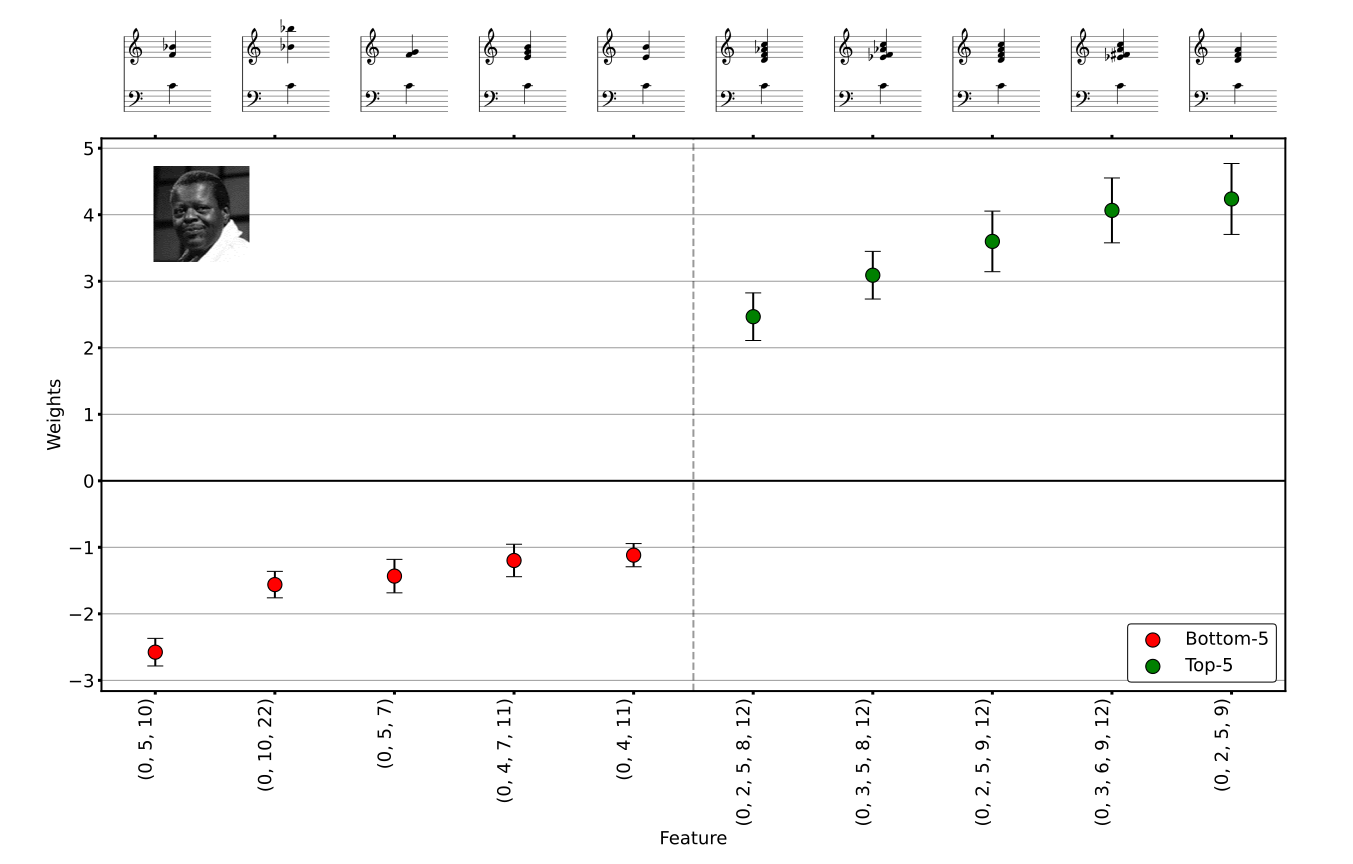
\includegraphics[width=1\textwidth]{figures/rsi_xai/figure_s37.pdf}
  \caption{Predictive harmony features, Oscar Peterson.}
\label{fig:rsi_sm_peterson_harmony}
\end{figure}

\begin{figure}[!ht]
  \centering
  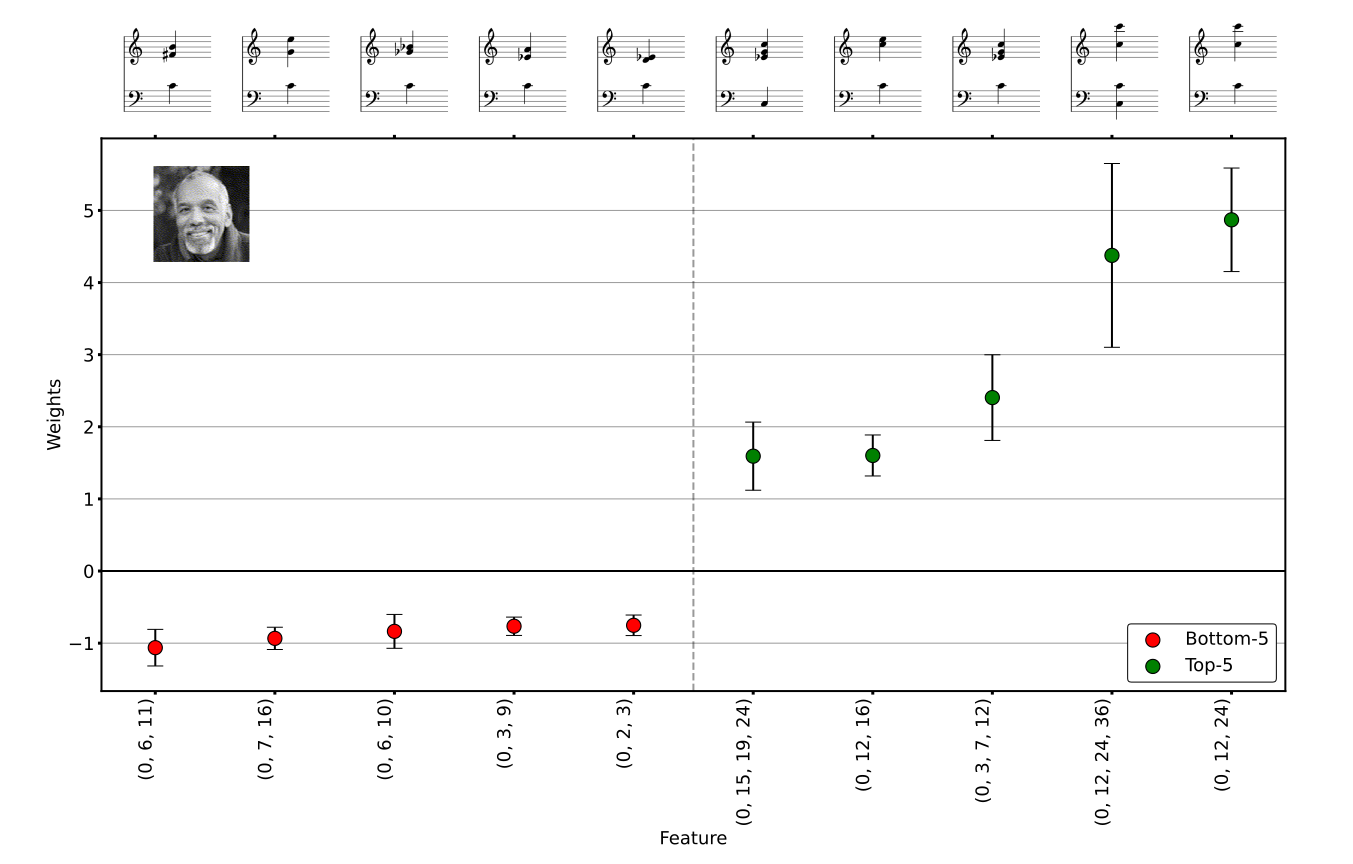
\includegraphics[width=1\textwidth]{figures/rsi_xai/figure_s38.pdf}
  \caption{Predictive harmony features, Stanley Cowell.}
\label{fig:rsi_sm_cowell_harmony}
\end{figure}

\begin{figure}[!ht]
  \centering
  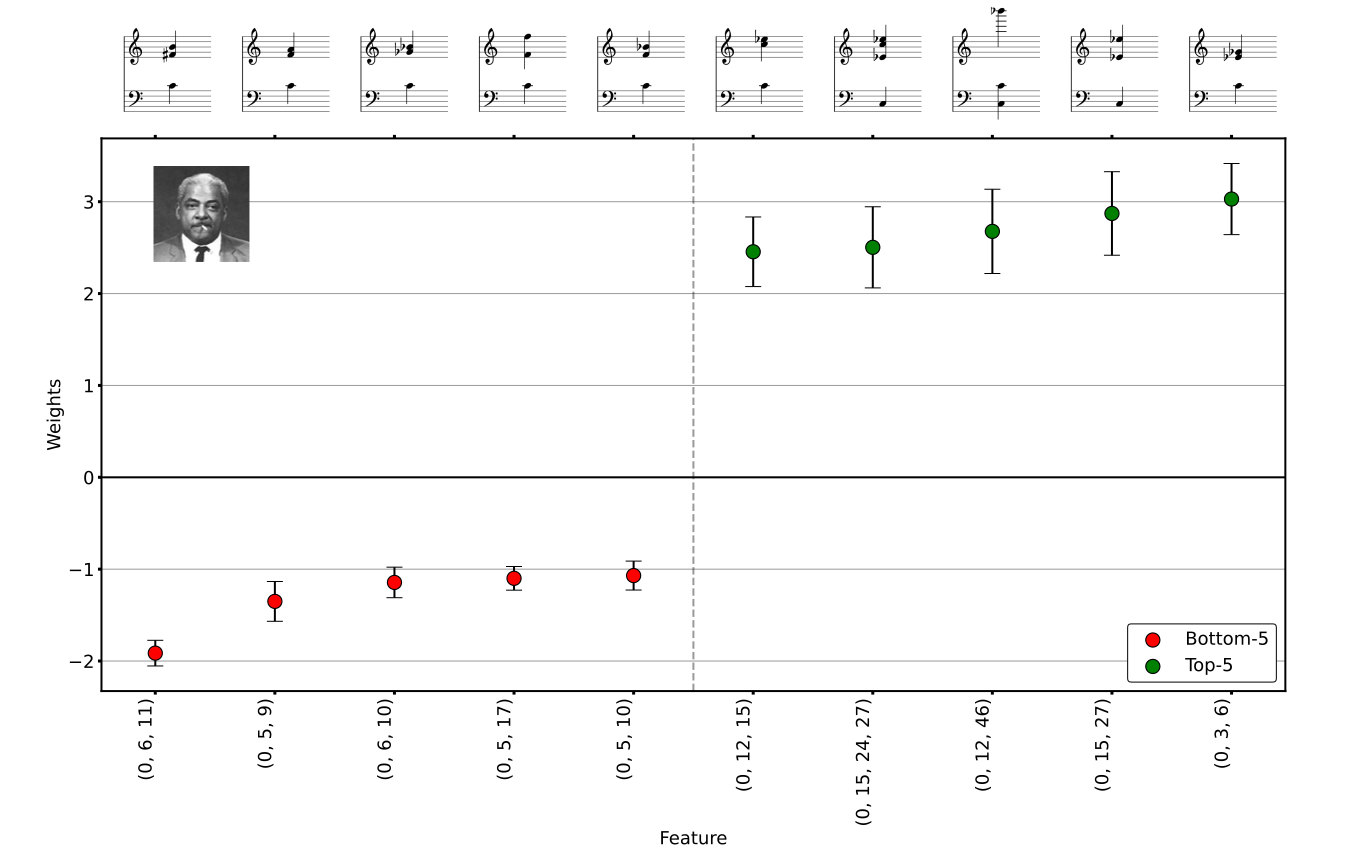
\includegraphics[width=1\textwidth]{figures/rsi_xai/figure_s39.pdf}
  \caption{Predictive harmony features, Teddy Wilson.}
\label{fig:rsi_sm_wilson_harmony}
\end{figure}

\begin{figure}[!ht]
  \centering
  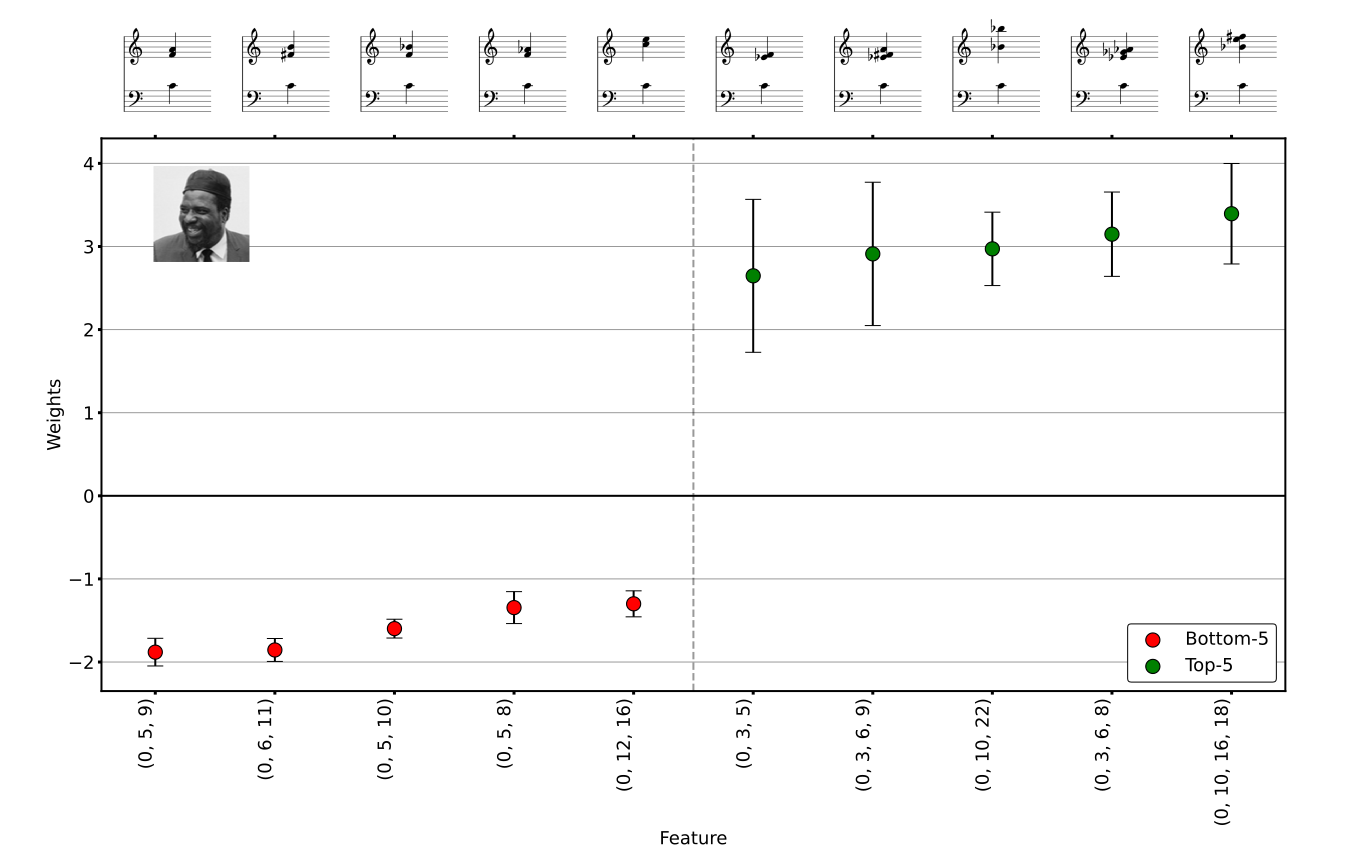
\includegraphics[width=1\textwidth]{figures/rsi_xai/figure_s40.pdf}
  \caption{Predictive harmony features, Thelonious Monk.}
\label{fig:rsi_sm_monk_harmony}
\end{figure}

\begin{figure}[!ht]
  \centering
  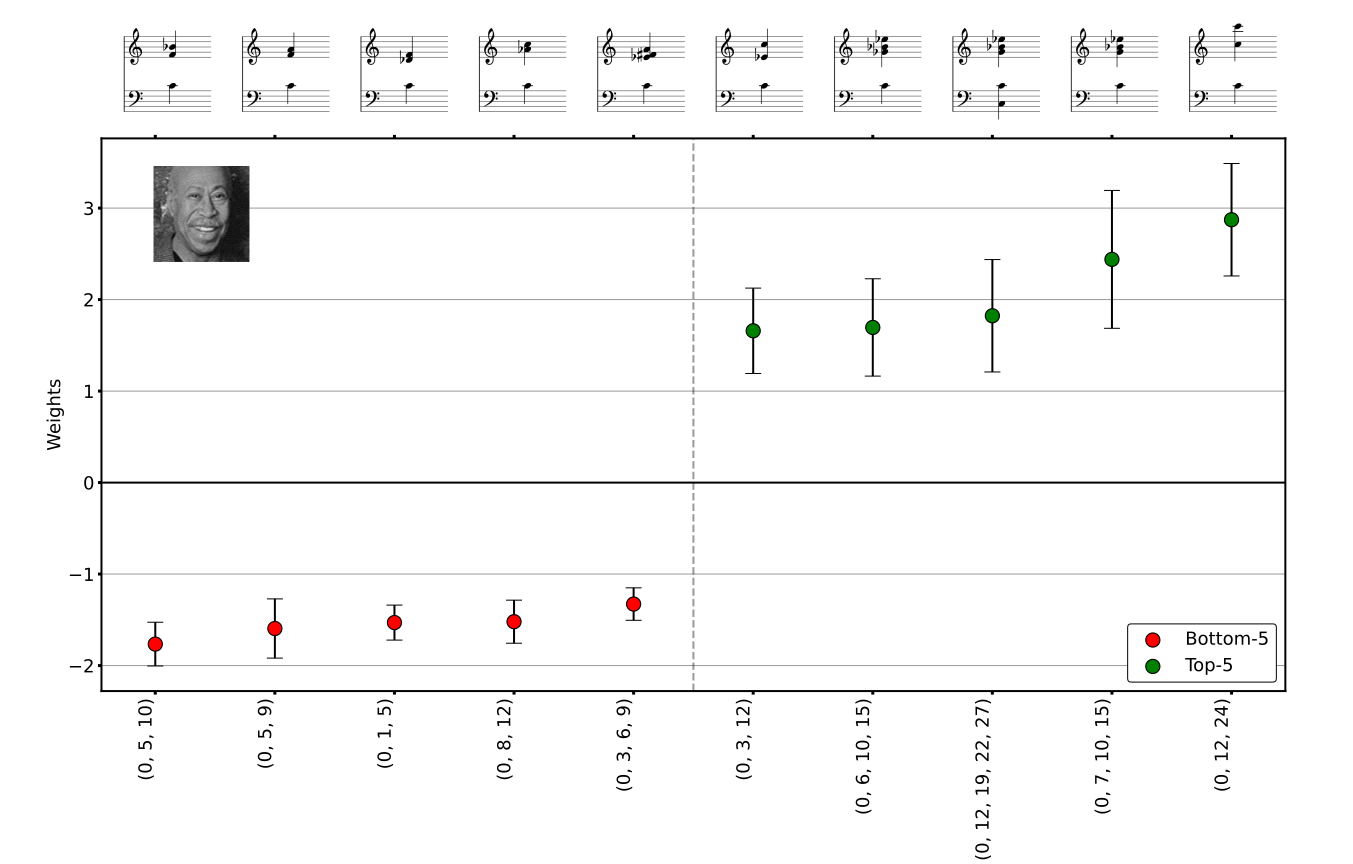
\includegraphics[width=1\textwidth]{figures/rsi_xai/figure_s41.pdf}
  \caption{Predictive harmony features, Tommy Flanagan.}
\label{fig:rsi_sm_flanagan_harmony}
\end{figure}

\begin{figure}[!ht]
  \centering
  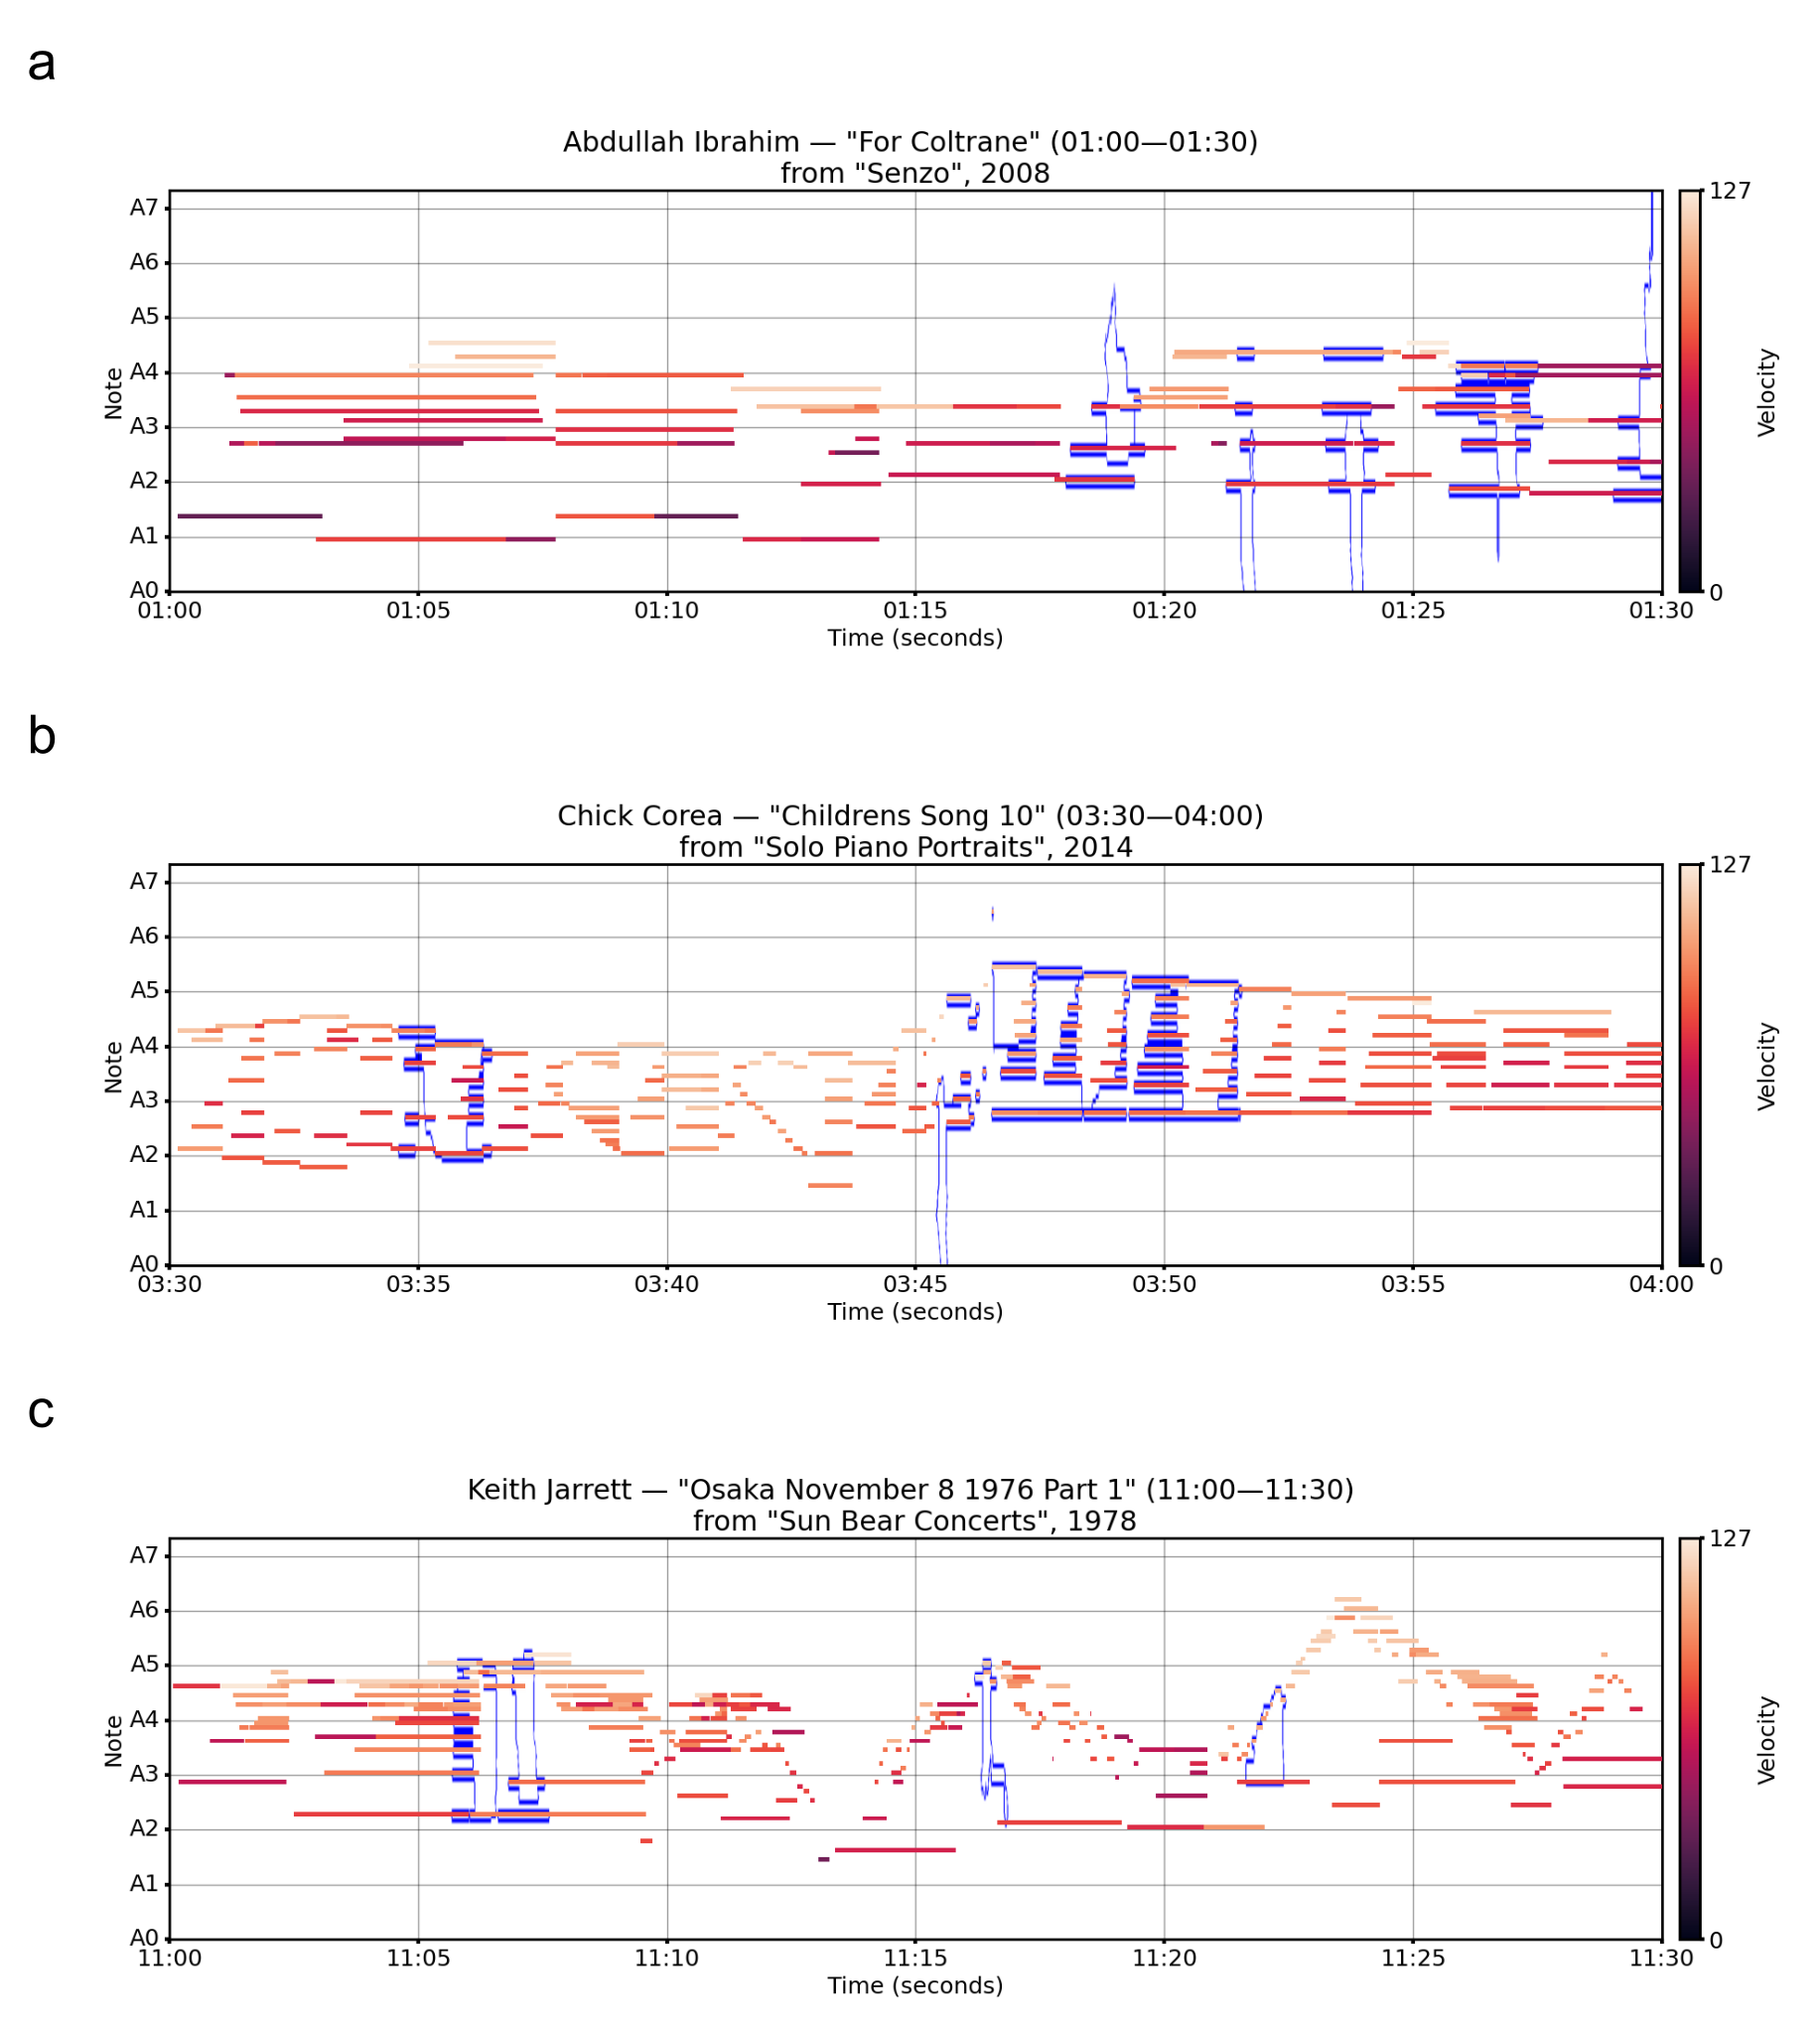
\includegraphics[width=1\textwidth]{figures/rsi_xai/figure_s42.pdf}
  \caption[Further masked piano rolls generated with \GLS{LIME}.]{Further masked piano rolls generated with \GLS{LIME}. Each panel shows a single 30-second clip from a transcription of a performance by (a) Abdullah Ibrahim, (b) Chick Corea, and (c) Keith Jarrett, taken from the held-out test split. Highlighted in blue are the top five areas of the piano roll that positively contribute to predicting the target label according to \GLS{LIME}.}
\label{fig:rsi_sm_lime_plots}
\end{figure}
